\documentclass[aspectratio=169]{beamer}

\usepackage[hyperref,backend=biber,
% Exemples de styles: alphabetic, ieee, nature, numeric, verbose-trad1 (en utilisant \footcite{}).
% https://www.overleaf.com/learn/latex/Biblatex_bibliography_styles
style=alphabetic,
% backref=true,
% backrefstyle=three,
]{biblatex}

\newif\ifwebcast
\webcastfalse
\newcommand{\webcast}{\webcasttrue}
% \webcast
% \newcommand<>{\script}[1]{\note#2{{#1}}}
% \newcommand<>{\script}[1]{\note{\only#2{#1}}}
\def\script{\note}

\definecolor{supelecRed}{RGB}{120,30,56}
\definecolor{supelecPurple}{RGB}{104,95,115}
\usetheme{Thesis}

\usepackage[utf8]{inputenc}
\usepackage[english]{babel}
\usepackage{tikz}
\usepackage{bm}
\usepackage{ulem}
\usepackage{parcolumns}
\usepackage{multicol}
\usepackage{booktabs}
\usepackage[french]{isodate}
\usepackage[ruled,noend,algo2e]{algorithm2e}
\usepackage[T1]{fontenc}
\usepackage{lmodern} % Assurer une bonne impression!
\usepackage{tikz} % tikz est utilise pour tracer des boites, par exemple
\usepackage{pgfplots}
\usepackage{fix-cm}
\usepackage{grffile}
\usepackage{pgfpages}
\usepackage{xparse}

\usepackage{pifont} % Pour utiliser des symboles divers.
\usepackage{color}
\usepackage{comment}
\usepackage{xargs}
\usepackage[author={Accacio}]{pdfcomment}

\usepackage{mathtools}
\usepackage{amsmath}
\usepackage{amsthm}
\usepackage{mathrsfs}
\usepackage{mathbbol}

\usepackage{eucal}

\usepackage{subcaption}
\usepackage{caption}
\captionsetup{justification=centering}
\usepackage{float}
\usepackage{array}

\usepackage{xr}
\usepackage{subfiles}
\usepackage[math]{blindtext}
\usepackage{ifthen} % Entrer valeurs bool\'{e}ennes et autres options
\usepackage{csquotes} % Assurer les guillemets français

\usepackage{nicefrac,xfrac}
\usepackage{etoolbox}
\usepackage{fontawesome}
\usepackage{mathabx}

\usepackage{animate}
\usepackage{colortbl}

\definecolor{mpc_agent}{RGB}{243, 146, 0} % logo necsys
\colorlet{mpc_agent}{supelecRed!90}
\definecolor{mpc_coordinator}{RGB}{235, 235, 235}
\colorlet{mpc_coordinator}{supelecRed!10}
\definecolor{mpc_green}{RGB}{98, 160, 98}
\newcommand\encircle[1]{%
  {
  \usebeamerfont*{item projected}%
  \usebeamercolor[bg]{item projected}%
  \begin{pgfpicture}{-1ex}{0ex}{1ex}{2ex}
    \pgfpathcircle{\pgfpoint{0pt}{.75ex}}{1.4ex}
    \pgfusepath{fill}
    \pgftext[base]{\color{fg}#1}
  \end{pgfpicture}%
  }
}

\newcommand{\tikzmark}[1]{\tikz[baseline={(#1.base)},overlay,remember picture] \node[outer sep=0pt, inner sep=0pt] (#1) {\phantom{A}};}

\newcommand{\booksymbol}{\lower4pt\hbox{\pgfuseimage{beamericonbook}}}
\tikzset{%
  show controls/.style={
    postaction={
      decoration={
        show path construction,
        curveto code={
          \draw [blue]
          (\tikzinputsegmentfirst) -- (\tikzinputsegmentsupporta)
          (\tikzinputsegmentlast) -- (\tikzinputsegmentsupportb);
          \fill [red, opacity=0.5]
          (\tikzinputsegmentsupporta) circle [radius=.2ex]
          (\tikzinputsegmentsupportb) circle [radius=.2ex];
        }
      },
      decorate
    }}}

\usetikzlibrary{graphs,quotes,graphs.standard}
\usetikzlibrary{plotmarks}
\usetikzlibrary{arrows.meta}
\usepgfplotslibrary{patchplots}
\usetikzlibrary{calc,shapes,positioning}
\usetikzlibrary{math}
\usetikzlibrary{overlay-beamer-styles}
\tikzset{
  graphs/nodes={draw,circle,inner sep=1pt},
  <->/.style={latex-latex},
  ->/.style={-latex},
  <-/.style={latex-},
}
\usetikzlibrary {chains}
\usetikzlibrary{arrows.meta}
\usetikzlibrary{3d}
\usetikzlibrary{perspective}
\usetikzlibrary{calc,shapes,positioning,intersections}
\usetikzlibrary{overlay-beamer-styles}
 \usetikzlibrary{plotmarks}
  \usetikzlibrary{arrows.meta}
\usetikzlibrary{babel} % to correct problem with babel

% \usepackage{times}
% Or whatever. Note that the encoding and the font should match. If T1
% does not look nice, try deleting the line with the fontenc.
\graphicspath{{../img/}}

\usepackage{amssymb}
\usepackage{accents}

\SetKwRepeat{Do}{do}{while}


\newcommand{\eq}[2]{\mbox{$#1=#2$}}
\newcommand{\N}{\mathbb{N}}
\newcommand{\Z}{\mathbb{Z}}
\newcommand{\Q}{\mathbb{Q}}
\newcommand{\R}{\mathbb{R}}
\newcommand{\C}{\mathbb{C}}
\newcommand{\Np}{N_{\text{p}}}
\newcommand{\T}{^{\mathrm{T}}}
\newcommand{\1}{\mathbf{1}}
\newcommand{\0}{\mathbf{0}}
\newcommand{\abs}[1]{\left\lvert#1\right\rvert}
\newcommand{\norm}[1]{\left\lVert#1\right\rVert}
\newcommand{\blkdiag}{\mathop{\rotatebox{90}{$\diameter$}}}

\newcommand{\vectorize}[1]{\mathrm{vec} (#1)}
\newcommand{\Varepsilon}{\mathcal{E}}
\newcommand{\diff}{\mathop{}\mathopen{}\mathrm{d}}
\newcommand{\set}[1]{\mathcal{#1}}
\newcommand{\graph}[1]{\mathscr{#1}}
\newcommand{\p}{^{(p)}}
\newcommand{\pplusone}{^{(p+1)}}
\newcommand{\h}{^{(h)}}
\newcommand{\hplusone}{^{(h+1)}}
\renewcommand{\vec}[1]{\boldsymbol{#1}}
\newcommand{\random}[1]{\underline{#1}}
\newcommand{\randomvec}[1]{{\underline{\vec{#1}}}}
\newcommand{\probability}[1]{\mathbb{P}(#1)}
\newcommand{\pdf}[1]{p(#1)}
\newcommand{\expectation}[2][]{\mathbb{E}_{#1}\left[#2\right]}
\newcommand{\indicator}[1]{\mathbb{1}_{\{#1\}}}
\newcommand{\vecangle}[2]{\langle_{#1}^{#2}}
\newcommand{\until}{\mathbin{:}}
\newcommand{\pseudoinv}[1]{{#1}^{\dagger}}


\newcommand{\setbuild}[2]{\{#1\mid#2\}}
\newcommand{\seq}[2][n]{\lbrace #2_{0},\ldots,\,#2_{#1} \rbrace}
\newcommand{\hadamard}[2]{#1\circ #2}
\newcommand{\kron}[2]{#1\otimes#2}
\newcommand{\symmetric}{\mathbb{S}}
\newcommand{\semidefpos}{\mathbb{S}_{+}}
\newcommand{\defpos}{\mathbb{S}_{++}}
\newcommand{\elem}[2][1]{{#2}_{(#1)}}
\renewcommand{\implies}{\Rightarrow}
\renewcommand{\iff}{\Leftrightarrow}
\newcommand{\argmax}{\mathop{\arg\!\max}}
\newcommand{\argmin}{\mathop{\arg\!\min}}
\newcommand{\maximize}{\mathop{\textrm{maximize}}}
\newcommand{\minimize}{\mathop{\textrm{minimize}}}
\newcommand{\minimiser}{\mathop{\textrm{minimiser}}}
\newcommand{\maximiser}{\mathop{\textrm{maximiser}}}

\DeclareMathOperator{\elemend}{end}
\DeclareMathOperator{\diag}{diag}
\DeclareMathOperator{\fix}{fix}
\DeclareMathOperator{\Proj}{Proj}
\DeclareMathOperator{\dom}{dom}
\DeclareMathOperator{\card}{\#}
% \DeclareMathOperator{\vectorize}{vector}
% \DeclareMathOperator{\vector}{vec}
%

% Theorem
% \newtheorem{thm}{Theorem}[section]
% \newtheorem{lem}[thm]{Lemma}

\newcommand{\nsubsystems}{M}
\newcommand{\umax}{\vec{u}_{\mathrm{\max}}}
\newcommand{\predhorz}{N}
\newcommand{\predictionSet}{\set{N}}
\newcommand{\nineq}{n_{\text{ineq}}}

\NewDocumentCommand \mpcvec { s m o o o } {%
  \IfBooleanTF{#1}{
    \def\optim{^\star}
  }{
    \def\optim{}
  }
  \IfValueTF{#5}{
    \vec{#2}_{#3}\optim{}[#4|#5]
  }{
    \IfValueTF{#4}{
      \vec{#2}_{#3}\optim{}[#4]
    }
    {
    \IfValueTF{#3}{
      \vec{#2}_i\optim{}[#3]
    }
    {
      \vec{#2}_i\optim{}[k]
    }
    }
  }
}


\NewDocumentCommand \mpcval { s m o o o } {%
  \IfBooleanTF{#1}{
    \def\optim{^\star}
  }{
    \def\optim{}
  }
  \IfValueTF{#5}{
    {#2}_{#3}\optim{}[#4|#5]
  }{
    \IfValueTF{#4}{
      {#2}_{#3}\optim{}[#4]
    }
    {
    \IfValueTF{#3}{
      {#2}_i\optim{}[#3]
    }
    {
      {#2}_i\optim{}[k]
    }
    }
  }
}






\newcommand{\uikk}{\mpcvec{u}[i][k][k]}
\newcommand{\optuikk}{\mpcvec*{u}[i][k][k]}

\newcommand{\globobj}{\mpcval{J}[][k]}
\newcommand{\optglobobj}{\mpcval*{J}[][k]}

\newcommand{\eqobj}{\bar{J}}
\newcommand{\eqoptobj}{\eqobj^{\star}}
\newcommand{\eqobji}{\eqobj_{i}}
\newcommand{\eqoptobji}{\eqobj_{i}^{\star}}
\newcommand{\obj}{J}
\newcommand{\optobj}{\obj^{\star}}
\newcommand{\obji}{\obj_{i}}
\newcommand{\optobji}{\obj_{i}^{\star}}
\newcommand{\Jacc}{\obj^{\text{acc}}}
\newcommand{\Jiacc}[1][i]{\obj_{#1}^{\text{acc}}}


\newcommand{\xik}{\mpcvec{x}}
\newcommand{\fik}{\mpcvec{f}}
\newcommand{\uik}{\mpcvec{u}}
\newcommand{\uiseq}{\mpcvec{u}[i][k:k+\predhorz-1][k]}
\newcommand{\optuiseq}{\mpcvec*{u}[i][k:k+\predhorz-1][k]}

\newcommand{\useq}{\mpcvec{u}[ ][k:k+\predhorz-1][k]}
\newcommand{\optuseq}{\mpcvec*{u}[ ][k:k+\predhorz-1][k]}
\newcommand{\Uik}{\mpcvec{U}}
\newcommand{\optUik}{\mpcvec*{U}}
\newcommand{\optuncUik}{\mpcvec*{\mathring{U}}}
\newcommand{\optuncU}{{\mathring{\vec{U}}^{\star}}}

\newcommand{\vik}{\mpcvec{v}}
\newcommand{\wik}{\mpcvec{w}}
\newcommand{\wiseq}{\mpcvec{w}[i][k:k+\predhorz-1][k]}
\newcommand{\Wik}{\mpcvec{W}}

\newcommand{\qik}{\mpcvec{q}}
\newcommand{\qiseq}{\mpcvec{q}[i][k:k+\predhorz-1][k]}
\newcommand{\thetaik}{\mpcvec{\theta}}
\newcommand{\optthetaiseq}{\mpcvec*{\theta}[i][k:k+\predhorz-1][k]}
\newcommand{\thetaseq}{\mpcvec{\theta}[][k:k+\predhorz-1][k]}
\newcommand{\optthetaseq}{\mpcvec*{\theta}[][k:k+\predhorz-1][k]}
\newcommand{\thetai}[1][i]{\vec{\theta}_{#1}}
\newcommand{\optthetai}{\vec{\theta}_i^{\star}}

\newcommand{\dik}{\mpcvec{d}}
\newcommand{\diseq}{\mpcvec{d}[i][k:k+\predhorz-1][k]}
\newcommand{\lambdaik}{\mpcvec{\lambda}}
\newcommand{\lambdaikstar}{\mpcvec*{\lambda}}
\newcommand{\lambdai}[1][i]{\vec{\lambda}_{#1}}
% \newcommand{\modified}[1]{\underaccent{\sim}{#1}}
\newcommand{\modified}[1]{\accentset{\text{mod}}{#1}}
\newcommand{\reconstructed}[1]{\accentset{\text{rec}}{#1}}
\newcommand{\lambdaimodified}{\modified{\vec{\lambda}}_{i}}
\newcommand{\lambdamodified}{\modified{\vec{\lambda}}}
\newcommand{\lambdaireconstructed}{\reconstructed{\vec{\lambda}}_{i}}
\newcommand{\lambdaicheat}{\tilde{\vec{\lambda}}_{i}}
\newcommand{\thetairestricted}{\overset{\scalebox{.5}{$\diameter$}}{\thetai}}

% \newcommand{\Tik}{\mpcval{T}}
\newcommand{\Tik}[1][i]{T_{#1}[k]}
\newcommand{\Tikinvestimate}[1][i]{\widehat{\Tik[#1]^{-1}}}
\newcommand{\Plin}[1][i]{{P}_{#1}}
\newcommand{\Plinnominal}[1][i]{\bar{{P}}_{#1}}
\newcommand{\Plintilde}[1][i]{\tilde{P}_{#1}[k]}
\newcommand{\Plintildeestimate}[1][i]{\widehat{\tilde{P}}_{#1}[k]}
\newcommandx*\Plinineq[2][1=i, 2=0]{\Plin[#1]^{\left(#2\right)}}
\newcommandx*\Plinineqnominal[2][1=i, 2=0]{\bar{\Plin[#1]}^{\left(#2\right)}}
\newcommandx*\Plinineqtilde[2][1=i, 2=0]{\widetilde{\Plin[#1]}^{\left(#2\right)}}
\newcommandx*\Plinineqtildeestimate[2][1=i, 2=0]{\widehat{\widetilde{\Plin[#1]}}^{\left(#2\right)}[k]}

\newcommand{\sik}[1][i]{\vec{s}_{#1}[k]}
\newcommand{\siktilde}[1][i]{\tilde{\vec{s}}_{#1}[k]}
\newcommand{\siktildeestimate}[1][i]{\widehat{\tilde{\vec{s}}}_{#1}[k]}
\newcommandx*\sikineq[2][1=i, 2=0]{\vec{s}_{#1}^{\left(#2\right)}[k]}
\newcommandx*\sikineqtilde[2][1=i, 2=0]{\widetilde{\vec{s}_{#1}}^{\left(#2\right)}[k]}
\newcommandx*\sikineqtildeestimate[2][1=i, 2=0]{\widehat{\widetilde{\vec{s}_{#1}}}^{\left(#2\right)}[k]}

\newcommand{\lagrangianname}{\mathscr{L}}
\newcommand{\lagrangian}{\lagrangianname(\vec{U}_{i}[k],\lambdaik,\thetaik)}
\newcommand{\dualfunctionname}{\mathscr{D}}
\newcommand{\dualfunction}{\dualfunctionname(\lambdaik,\thetaik)}
\newcommand{\inequalityfunctionname}{g_i}
\newcommand{\inequalityfunction}{\inequalityfunctionname(\vec{U}_{i}[k],\thetaik)}
\newcommand{\equalityfunctionname}{h_i}
\newcommand{\equalityfunction}{\equalityfunctionname(\vec{U}_{i}[k],\thetaik)}
\newcommand{\linearcoefi}{\bar{\Gamma}_{i}H_{i}^{-1}\bar{\Gamma_{i}}^{T}}
\newcommand{\linearcoefiineqnonzero}[1][\star,\star]{\elem[#1]{\bar{\Gamma}_{i}}H_{i}^{-1}{(\elem[#1]{\bar{\Gamma}_{i}})}^{T}}

\newcommand{\rlsparam}{{\vec{\nu}_{i}}}
\newcommand{\rlssysinput}{{B_i}}
\newcommand{\rlssysoutput}{{\lambdai}}
\newcommand{\rlsgain}{{\Phi}}
\newcommand{\rlsforget}{{\phi}}
\newcommand{\rlsresidual}{{\epsilon}}

\newcommand{\pwaestparam}{{\vec{\nu}}}
\newcommand{\pwaestnumparam}{{n}}
\newcommand{\pwaestsysinput}{{B}}
\newcommand{\pwaestsysoutput}{{\vec{\gamma}}}
\newcommand{\pwaestgain}{{\Phi}}
\newcommand{\pwaestforget}{{\phi}}
\newcommand{\pwaestresidual}{{\epsilon}}
\newcommand{\pwaestinputsize}{{N}}


\SetKwProg{Fn}{}{}{}
\SetKwFunction{structDataSym}{structDataSym}%
\SetKwBlock{coordinit}{ Coordinator initialization:}{}
\SetKwBlock{exchange}{ Exchange between Coordinator and agents:}{}
\SetKwBlock{negotPhase}{ Negotiation Phase:}{}
\SetKwBlock{detectPhase}{ Detection Phase:}{}

\SetKwBlock{coordinitfr}{ Initialisation du Coordinateur:}{}
\SetKwBlock{exchangefr}{ Échange entre Coordinateur et agents:}{}
\SetKwBlock{negotPhasefr}{ Phase de Négociation:}{}
\SetKwBlock{detectPhasefr}{ Phase de Détection:}{}
\SetKwIF{Si}{SinonSi}{Sinon}{si}{alors}{sinon si}{sinon}{}
\SetKwFor{Tq}{tant que}{faire}{fintq}
\SetKwRepeat{Repeter}{répéter}{jusqu’à}
\SetKwInput{Entree}{Entrées}
\SetKwInput{Sortie}{Sorties}


\newtheorem{assumption}{Assumption}%[numberby]
\newtheorem{assumptions}[assumption]{Assumptions}
\newtheorem{remark}{Remark}

\newif\ifdebug%
\newcommand{\draft}{\debugtrue}
\newcommand{\final}{\debugfalse}
\newcommand{\todo}[2][FORGOT TO DO SOMETHING]{\ifdebug%
  {%
    \color{red}
    #2}\else \PackageError{}{#1}{#2}#2\fi}%
\newcommand\doing[2][FORGOT TO DO SOMETHING]{\ifdebug%
  {%
    \color{blue}
    #2}\else \PackageError{}{#1}{#2}#2\fi}%
\newcommand\warning[1]{\ifdebug%
  {%
    \color{red}
    #1}\fi}


% \setbeameroption{show notes on second screen}
\draft
% \webcast
\setbeamercolor{alerted text}{fg=supelecRed!20!red!80}
% \usetikzlibrary{overlay-beamer-styles}
\bibliography{../tex/bibliography.bib}

\title[Security of dMPC under False Data Injection] % (optional, use only with long paper titles)
{Security of distributed Model Predictive Control\\ under False Data Injection}

% \subtitle
% {or How I Learned to Stop and Worry about Everything}

\author[Rafael Accácio Nogueira] % (optional, use only with lots of authors)
{Rafael Accácio NOGUEIRA}

\institute[IETR --- CentraleSupélec] % (optional, but mostly needed)
{
}

\day12 \month12 \year2022
\date
{
  2022-12-12\\
  \begin{minipage}{.3\textwidth}
    \centering
    
\includegraphics[width=2cm]{logos/IETR_2022.png}
  \end{minipage}
  \hfill
  \begin{minipage}{.3\textwidth}
    \centering
    \vspace{10pt}
    
\includegraphics[width=1.5cm]{qrPresentation.png}
    % qrencode https://github.com/Accacio/thesis/raw/main/presentation/presentation.pdf -o ~/git/SysTol21/img/qrPresentation.png
    \href{https://bit.ly/3g3S6X4}{https://bit.ly/3g3S6X4}
  \end{minipage}
  \begin{minipage}{.3\textwidth}
    \centering
    \vspace{10pt}
    
\includegraphics[width=2cm]{logos/supelec.jpeg}
  \end{minipage}
}
% - Either use conference name or its abbreviation.
% - Not really informative to the audience, more for people (including
%   yourself) who are reading the slides online

\subject{}

\logo{
\includegraphics[width=1.5cm]{logos/supelec.jpeg}}

% Delete this, if you do not want the table of contents to pop up at
% the beginning of each subsection:
\AtBeginSection[]
{
  \begin{frame}<beamer>{Outline}
    \tableofcontents[sectionstyle=show/hide,subsectionstyle=show/show/hide]
  \end{frame}
}

\begin{document}

\begin{frame}[plain]
  % \frametitle{Ph.D. Defense}
  \titlepage%
  \note{45 minutes !!!!\\}
  \script{Good afternoon, thank you all for being here.}
  \script{I'm Rafael Accácio and I'm going to present my work on the security of distributed model predictive control under false data injection.}
\end{frame}

\begin{frame}{Context}{\raisebox{0.1cm}{\scalebox{0.5}{\faQuoteLeft\ }}Necessity is the mother of invention\raisebox{0.1cm}{\scalebox{0.5}{\ \faQuoteRight}}}
  % \only<6>{
  % Smart City\\}
  \only<1>{
    \centering
    \begin{tikzpicture}
      \node (image) at (0,0) {\includegraphics<1>[width=0.5\textwidth]{city_grass_layer.pdf}};
      \node (image) at (0,0) {\includegraphics<1>[width=0.5\textwidth]{city_streets_layer.pdf}};
      \node (image) at (0,0) {\includegraphics<1>[width=0.5\textwidth]{city_houses_layer.pdf}};
      \node (image) at (0,0) {\includegraphics<1>[width=0.5\textwidth]{city_buildings_layer.pdf}};
      \node (image) at (0,0) {\includegraphics<1>[width=0.5\textwidth]{city_trees_layer.pdf}};
    \end{tikzpicture}


  }
  \only<2->{
    \begin{minipage}{.45\textwidth}
      \centering

      \begin{tikzpicture}
        \node (image) at (0,0) {\includegraphics<2->[width=\textwidth]{city_grass_layer.pdf}};
        \node (image) at (0,0) {\includegraphics<2->[width=\textwidth]{city_streets_layer.pdf}};
        \node (image) at (0,0) {\includegraphics<2->[width=\textwidth]{city_houses_layer.pdf}};
        \node (image) at (0,0) {\includegraphics<2->[width=\textwidth]{city_buildings_layer.pdf}};
        \node (image) at (0,0) {\includegraphics<2->[width=\textwidth]{city_trees_layer.pdf}};
        \node (image) at (0,0) {\includegraphics<3->[width=\textwidth]{city_energy_layer.pdf}};
        \node (image) at (0,0) {\includegraphics<4->[width=\textwidth]{city_heat_water_layer.pdf}};
        \node (image) at (0,0) {\includegraphics<5->[width=\textwidth]{city_cars_layer.pdf}};
      \end{tikzpicture}
    \end{minipage}
    \hfill
    \only<3-6>{
      \begin{minipage}{.5\textwidth}
        \begin{itemize}
          \item<3-> Electricity Distribution System
          \item<4-> Heat distribution
          \item<4-> Water distribution\\
          \item<5-> Traffic management
          \item[]<6->(include your problem here)
        \end{itemize}
      \end{minipage}
    }
    \only<7->{
      \begin{minipage}{.5\textwidth}
        \begin{itemize}
          \item<7-> Multiple systems interacting
          \item<8-> Coupled by constraints
                \begin{itemize}[<+(1)->]
                  \item<9-> Technical/ Comfort
                \end{itemize}
          \item<10-> Optimization objectives
                \begin{itemize}[<+(1)->]
                  \item<11-> Minimize energy consumption
                  \item<12-> Maximize user satisfaction
                  \item<13-> Follow a trajectory
                \end{itemize}
          \item<14-> Solution $\to$ MPC
        \end{itemize}
      \end{minipage}
    }

  }
  % \script<5->{The systems are usually }
  % \script<5->{Geographically distributed }
  % \script<6->{Coupled by constraints as maximum input power or energy }
  % \script<7->{and when they are implemented we try to optimize objectives such as cost, energy, user satisfaction and others.\\ }
  % \script<8>{A solution is to use MPC}
  % \script{These cyberphysical systems are the majority of the systems in our everyday lives.}
  % \script{We can give example the traffic management,}
  % \script{water distribution,}
  % \script{electricity distribution, heat and cold and many more.}

  % \script{But how to control those kinds of systems.}
  % \script{Each has its own Dynamics and constraints,  such comfort (Quality of service) or technical.}
  % \script{Solution, mpc since we use models and it is easy to integrate the constraints.}

\end{frame}

\begin{frame}{Model-based Predictive Control}
  \pause
  Find \only<1-3>{\alert<3>{best}}\only<4->{optimal} control sequence using predictions based on a model.
  \begin{itemize}
    \item<5-> We need an optimization problem
          \begin{itemize}
            \item<6-> Decision variable is the control sequence \only<7->{(Over horizon N)}
            \item<8-> Objective function to optimize
            \item<9-> System's Model (\alert<10>{states} and \alert<11>{inputs})
            \item<12-> Other constraints to respect \onslide<13->{(QoS, technical restrictions, ...)}
          \end{itemize}
  \end{itemize}
  \vspace{1cm}
  % \only<4-12>{
  \visible<5->{
    \begin{equation*}
      \begin{matrix}
        \minimize\limits_{\alert<6>{\vec{u}[0:\alert<7>{\predhorz}-1|k]}} & \alert<8>{J(\vec{x}[0|k],\vec{u}[0:\alert<7>{\predhorz}-1|k])}&\\
        \onslide<9->{\mathrm{subject~ to} &
                                            \left.
                                            \begin{matrix}
                                              \alert<10>{\vec{x}[\xi|k]}=f(\alert<10>{\vec{x}[\xi-1|k]},\alert<11>{\vec{u}[\xi-1|k]})\\
                                              \onslide<12-13>{\alert<12>{g_{i}(\vec{x}[\xi-1|k],\vec{u}[\xi-1|k])\leq0}}\\
                                              \onslide<12-13>{\alert<12>{h_{j}(\vec{x}[\xi-1|k],\vec{u}[\xi-1|k])=0}}\\
                                            \end{matrix}
        \right\}
        \begin{aligned}
          &\forall \xi\in\{1,\dots,\alert<5>{\predhorz}\}\\
          &\onslide<12-13>{\alert<12>{\forall i\in\{1,\dots,m\}}}\\
          &\onslide<12-13>{\alert<12>{\forall j\in\{1,\dots,p\}}}
        \end{aligned}}
      \end{matrix}
    \end{equation*}
    % }
  }%
  \script<1>{For those who are not familiar with mpc. Mpc is the model based predictive controller.}
  \script<2>{The objective is to find the best control sequence using predictions based on a model.}
  \script<3>{When we say best,}
  \script<4>{we mean optimal.}
  \script<5>{So we need to solve an optimization problem.}
  \script<6>{And we have the control sequence of u as the decision variable.}
  \script<7>{which is calculated for a horizon N}
  \script<8>{So, we need an objective function. For example follow a trajectory while minimizing the energy.}
  \script<9>{A model of the system}
  \script<10>{with its states }
  \script<11>{and inputs }
  \script<12>{But we can also integrate some constraints, such QoS or technical restrictions}

\end{frame}

% \begin{frame}{Context}
%   \begin{figure}
%     \includegraphics<1>[width=.6\textwidth]{the_city_nothing.pdf}%
%     \includegraphics<2>[width=.6\textwidth]{the_city_houses.pdf}%
%     \includegraphics<3>[width=.6\textwidth]{the_city_buildings.pdf}%
%     \includegraphics<4>[width=.6\textwidth]{the_city_cars.pdf}%
%   \end{figure}
%   \only<5->{
%   \begin{minipage}{.45\textwidth}
%     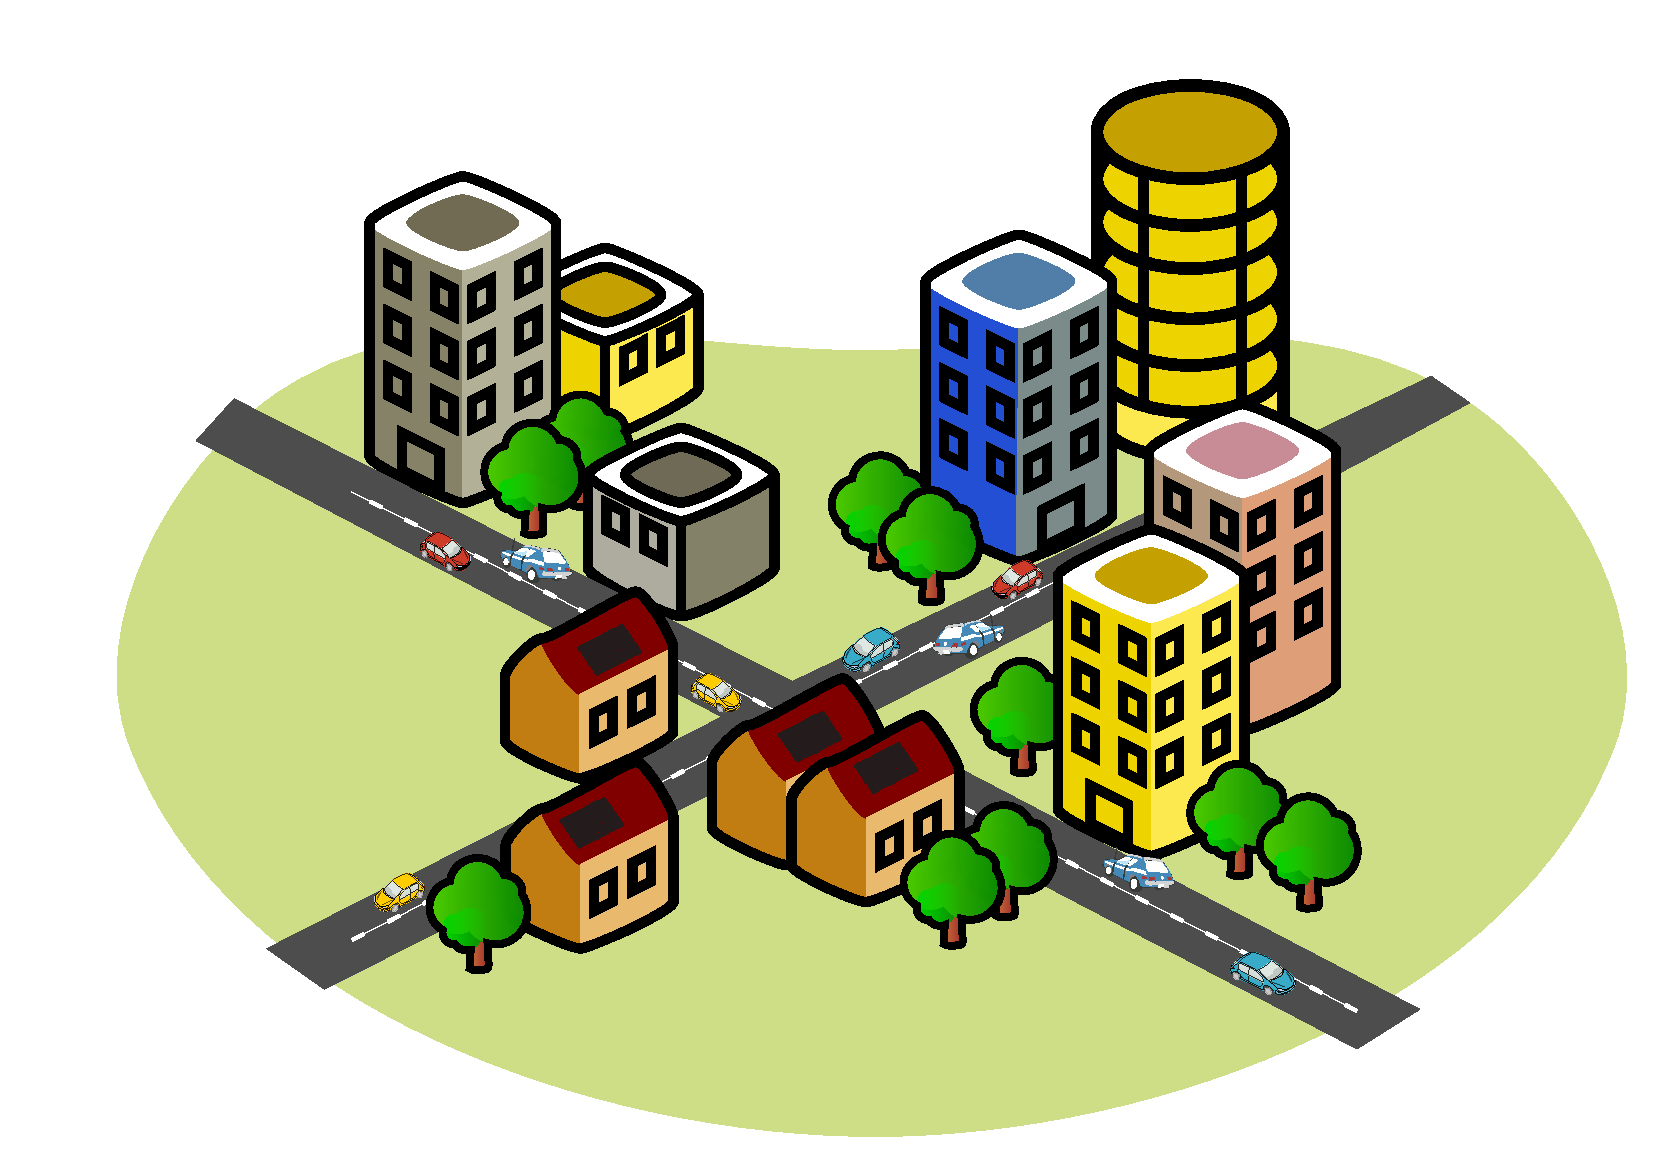
\includegraphics[width=\textwidth]{the_city_cars.pdf}%
%   \end{minipage}
%   \begin{minipage}{.5\textwidth}
%     \begin{itemize}
%       \item<6> Geographically distributed
%       \item<7> Coupled by constraints (energy)
%       \item<8> Optimization objectives
%       \begin{itemize}
%         \item Energy
%         \item User satisfaction
%         \item \dots
%       \end{itemize}
%       \item<9> Solution $\to$ Model Predictive Control
%     \end{itemize}
%   \end{minipage}
% }
% \end{frame}


% % \begin{frame}{Model Predictive Control}
% %   Objective: Find control input sequence that optimizes an objective function
% %   \only<1-5>{\begin{equation*}
% %     \begin{matrix}
% %       \underset{\vec{u}(k:k+\alert<3>{N_{p}}-1|k)}{\mathrm{optimize}}&\alert<2>{J(\vec{x}(k),\vec{u}(k))}\\
% %       \mathrm{subject~ to}&
% %       \left.
% %         \begin{matrix}
% %           \alert<4>{\vec{x}(\xi+1)=f(\vec{x}(\xi),\vec{u}(\xi))}\\
% %           \alert<5>{g_{i}(\vec{x}(\xi),\vec{u}(\xi))\leq0}\\
% %           \alert<5>{h_{j}(\vec{x}(\xi),\vec{u}(\xi))=0}\\
% %         \end{matrix}
% %       \right\}
% %       \begin{aligned}
% %         &\forall \xi\in\{1,\dots,\alert<3>{N_{p}}\}\\
% %         &\forall i\in\{1,\dots,m\}\\
% %         &\forall j\in\{1,\dots,p\}
% %       \end{aligned}
% %     \end{matrix}
% %   \end{equation*}}%
% %   \only<6->{
% %   \begin{equation*}
% %     \begin{matrix}
% %       \underset{\vec{u}(k:k+N_{p}-1|k)}{\mathrm{minimize}}&  \sum_{j=1}^{N_{p}}\|\vec{v}(k+j|k)\|^{2}_{Q}+\|\vec{u}(k+j-1|k)\|^{2}_{R}\\
% %       \mathrm{subject~ to}&
% %       \left.
% %         \begin{matrix}
% %           \vec{x}(\xi+1)=f(\vec{x}(\xi),\vec{u}(\xi)) \\
% %           g_{i}(\vec{x}(\xi),\vec{u}(\xi))\leq0\\
% %           h_{j}(\vec{x}(\xi),\vec{u}(\xi))=0\\
% %         \end{matrix}
% %       \right\}
% %       \begin{aligned}
% %         &\forall \xi\in\{1,\dots,N_{p}\}\\
% %         &\forall i\in\{1,\dots,m\}\\
% %         &\forall j\in\{1,\dots,p\}
% %       \end{aligned}
% %     \end{matrix}
% %   \end{equation*}
% % }%
% %   \script<1->{The Model based Predictive Control, for those who don't know is a control strategy where the control is computed by solving an optimization problem }
% %   \script<2->{with cost J. }
% %   \script<3->{The system's response for the input u is predicted for a period Np, }
% %   \script<4->{using the model of the system. }
% %   \script<5->{And we then add the equality and inequality constraints. }
% %   \script<6->{Usually the optimization problem is to minimize a quadratic objective function.}
% % \end{frame}

\newlength\fheight
\newlength\fwidth
\setlength\fwidth{.35\textwidth}
\setlength\fheight{.8\fwidth}

\begin{frame}{Model Predictive Control}{In a nutshell}
  \small
  \begin{overlayarea}{\textwidth}{\textwidth}
    \onslide<2->{Find optimal control sequence}%
    \only<3->{, apply first element}%
    \only<4->{, rinse repeat}%
    \only<5->{ $\to$ Receding Horizon}%

    \begin{figure}
      \centering
      \foreach \i in {1,...,6}{%
        % \includegraphics<\i>[width=.5\textwidth]{mpc\i.pdf}%
        \only<{\i}>{\input{../img/mpcState\i.tex}}%
        \only<{\i}>{\input{../img/mpcControl\i.tex}}%
      }
    \end{figure}
  \end{overlayarea}
  \script<1>{So, for example, if we may have a setpoint to follow}
  \script<2>{We find an optimal control sequence }
  \script<3>{We apply only the first element }
  \script<4>{and then we repeat }
  \script<5>{following what we call the receding horizon strategy.}
  \script<5>{However this problem is not always straightforward to solve, for some cases it can be easier.}

\end{frame}

\begin{frame}{Model Predictive Control}{Nothing is perfect}
  \begin{itemize}[<+(1)->]
    \item Problems
          \begin{itemize}
            \item Complexity of calculation
            \item Topology (Geographical distribution)
            \item Flexibility (Add/remove parts)
            \item Privacy
          \end{itemize}
    \item Solution: Divide and Conquer (distributed MPC)
          \begin{itemize}
            \item Break calculation
            \item Make agents communicate
          \end{itemize}
  \end{itemize}
\end{frame}

\begin{frame}{Distributed Model Predictive Control}{It is about communication}
  \begin{itemize}
    \item<.-> We break the MPC into multiple
    \item<+-> Make agents communicate. \only<+->{ But how?}
          \begin{itemize}
            \item<+-> Many flavors to choose from\visible<.(5)->{\footnote<.(5)->{{{\booksymbol~\citetitle{MaestreEtAl2014}}}}}
                  \begin{itemize}[<+->]
                    \item \alert<.(5)>{Hierarchical}/Anarchical
                    \item Sequential/Parallel
                    \item \alert<.(3)>{Synchronous}/Asynchronous
                    \item \alert<.(2)>{Bidirectional}/Unidirectional
                    \item ...
                  \end{itemize}
          \end{itemize}
  \end{itemize}
  \begin{minipage}[c]{.225\textwidth}
    \centering
    \onslide<4->{
      \scalebox{.45}{
        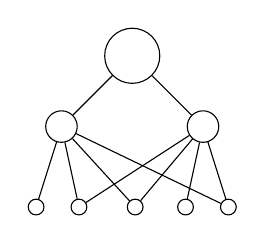
\begin{tikzpicture}[node distance=.5cm and .5cm,inner sep=0pt,every node/.style={minimum width=0.1cm}]
          \node[draw,circle,minimum width=.7cm] at (0,0) (first) {};
          \node[draw,circle,below left=of first,minimum width=.4cm] (second_l) {};
          \node[draw,circle,below right=of first,minimum width=.4cm] (second_r) {};

          \node[draw,circle,below left =0.8cm and 0.1cm  of second_l,minimum width=.2cm] (third_1) {};
          \node[draw,circle,below right=0.8cm and -0.0cm of second_l,minimum width=.2cm] (third_2) {};
          \node[draw,circle,right      =1.8cm and 0.5cm    of third_2   ,minimum width=.2cm] (third_3) {};
          \node[draw,circle,below left =0.8cm and -0.0cm of second_r,minimum width=.2cm] (third_4) {};
          \node[draw,circle,below right=0.8cm and 0.1cm  of second_r,minimum width=.2cm] (third_5) {};

          \draw[-]  (first)  -- (second_l);
          \draw[-]  (first)  -- (second_r);
          \draw[-]  (second_l) -- (third_1);
          \draw[-]  (second_l) -- (third_2);
          \draw[-]  (second_l) -- (third_3);
          \draw[-]  (second_l) -- (third_5);
          \draw[-]  (second_r) -- (third_2);
          \draw[-]  (second_r) -- (third_3);
          \draw[-]  (second_r) -- (third_4);
          \draw[-]  (second_r) -- (third_5);
        \end{tikzpicture}}

      \scalebox{.45}{
        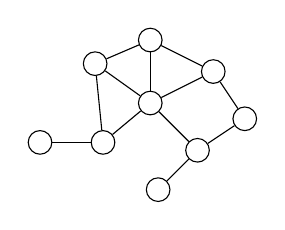
\begin{tikzpicture}[node distance=.5cm and .5cm,inner sep=0pt,every node/.style={minimum width=0.3cm}]
          \node[draw,circle] at (0,0) (a) {};
          \node[draw,circle] at ($(a)+(-.7,-.3)$) (b) {};
          \node[draw,circle] at ($(a)+(0.0,-0.8)$) (c) {};
          \node[draw,circle] at ($(a)+(0.8,-0.4)$) (d) {};
          \node[draw,circle] at ($(b)+(0.1,-1.0)$) (e) {};
          \node[draw,circle] at ($(e)+(1.2,-0.1)$) (f) {};
          \node[draw,circle] at ($(f)+(0.6,0.4)$) (g) {};
          \node[draw,circle] at ($(e)+(-0.8,-0.0)$) (h) {};
          \node[draw,circle] at ($(f)+(-0.5,-0.5)$) (i) {};

          \draw[-]  (a)  -- (b);
          \draw[-]  (a)  -- (c);
          \draw[-]  (a)  -- (d);
          \draw[-]  (b)  -- (c);
          \draw[-]  (c)  -- (d);
          \draw[-]  (e)  -- (b);
          \draw[-]  (e)  -- (c);
          \draw[-]  (c)  -- (f);
          \draw[-]  (d)  -- (g);
          \draw[-]  (f)  -- (g);
          \draw[-]  (e)  -- (h);
          \draw[-]  (f)  -- (i);
        \end{tikzpicture}}
    }
  \end{minipage}
  \hfill
  \begin{minipage}[c]{.225\textwidth}
    \centering
    \onslide<5->{
      \scalebox{.6}{
        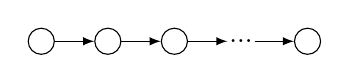
\begin{tikzpicture}[node distance=1cm and .5cm]
          \node[draw,circle] (first) at (0,0) {};
          \node[draw,circle,right=of first] (second) {};
          \node[draw,circle,right=of second] (third) {};
          \node[draw,circle,opacity=0,right=of third] (fourth) {};
          \node[draw,circle,right=of fourth] (fifth) {};

          \node[] at (fourth) {...};
          \draw[-latex] (first) -- (second);
          \draw[-latex] (second) -- (third);
          \draw[-latex] (third) -- (fourth);
          \draw[-latex] (fourth) -- (fifth);
        \end{tikzpicture}}

      \vspace{.5cm}
      \scalebox{.4}{
        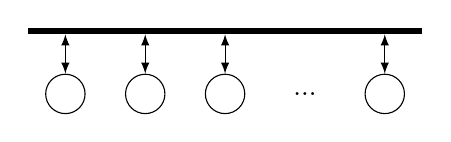
\begin{tikzpicture}[node distance=.5cm and .5cm,inner sep=0pt,minimum width=.5cm]
          \node[draw,rectangle,fill=black,minimum height=2pt,minimum width=5cm] (bar) at (0,0) {};
          % \draw[blue,fill] ($(bar)+(-2.5cm,-2pt)$) rectangle ($(bar)+(2.5cm,2pt)$);
          \node[draw,circle,below=of bar] (third) {};
          \node[draw,circle,left=of third] (second) {};
          \node[draw,circle,left=of second] (first) {};
          \node[draw,circle,opacity=0,right=of third] (fourth) {};
          \node[draw,circle,right=of fourth] (fifth) {};

          \node[] at (fourth) {...};
          \draw[latex-latex]  (first)  -- (bar.south -| first);
          \draw[latex-latex]  (second) -- (bar.south -| second);
          \draw[latex-latex]  (third)  -- (bar.south -| third);
          \draw[latex-latex]  (fifth)  -- (bar.south -| fifth);
        \end{tikzpicture}
      }}
  \end{minipage}
  \hfill
  \begin{minipage}[c]{.225\textwidth}
    \centering
    \tikzset{lightning bolt to/.style={to path={
let \p1=(\tikztostart), \p2=(\tikztotarget), \n1={veclen(\y2-\y1,\x2-\x1)} in
  (\p1) -- ($($(\p1)!0.6!(\p2)$)!\n1*.1!-90:(\p2)$) -- ($(\p1)!0.55!(\p2)$) --
  (\p2) -- ($($(\p1)!0.4!(\p2)$)!\n1*.1!90:(\p2)$) -- ($(\p1)!0.45!(\p2)$) --
  cycle (\p2)% Move to end point
}}}
    \onslide<6->{
        \begin{tikzpicture}
          \draw[fill,yellow!40!orange] (1,0) to [lightning bolt to] ++ (0,.5);
          \draw[fill,yellow!40!orange] (2,0) to [lightning bolt to] ++ (0,.5);
          \draw (0.5,0) -- (2.5,0);
        \end{tikzpicture}

        \vspace{.1cm}
        \begin{tikzpicture}
          \draw[fill,yellow!40!orange] (1,0) to [lightning bolt to] ++ (0,.5);
          \draw[yellow!40!orange] (2,0.25) to [lightning bolt to] ++ (0,.5);
          \draw (0.5,0) -- (2.5,0);
        \end{tikzpicture}
    }
  \end{minipage}
  \hfill
  \begin{minipage}[c]{.225\textwidth}
    \centering
    \onslide<7->{\scalebox{1}{
        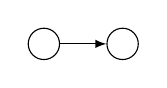
\begin{tikzpicture}
          \graph[empty nodes,nodes={inner sep=4pt}] {
            a -> b
          };
        \end{tikzpicture}}

      \vspace{.5cm}
      \scalebox{1}{
        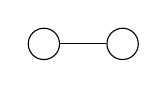
\begin{tikzpicture}
          \graph[empty nodes,nodes={inner sep=4pt}] {
            a -- b
          };
        \end{tikzpicture}
      }}
  \end{minipage}
  \begin{tikzpicture}[overlay, remember picture,decoration={brace,amplitude=2pt}]
  %   \node[] at (-2,3) {\includegraphics<6>[width=.35\textwidth]{nazare/0.png}};
  %   \node[] at (-2,3) {\includegraphics<7>[width=.35\textwidth]{nazare/12.png}};
    \node[] at (-1.5,3) {\includegraphics<6>[width=.3\textwidth]{nazare/42.png}};
    \node[] at (-1.5,3) {\includegraphics<7->[width=.3\textwidth]{nazare/64.png}};
  \end{tikzpicture}%
  \script<1>{However, the solution will depend on the horizon, the number of constraints, and sizes of input and states, increasing the complexity of the calculation }
  \script<2>{A strategy to alleviate is to distribute the calculation whenever possible. And there are many ways to divide it as the book shows.}
  \script<3>{Here we opt for a hierarchical strategy where we use multiple MPCs and an agent to coordinate and manage the coupling aspects of the problem.}
\end{frame}

\begin{frame}{Distributed Model Predictive Control}{Communication Frameworks}
  \begin{minipage}[c]{.45\linewidth}
    \begin{figure}[H]
      \centering
      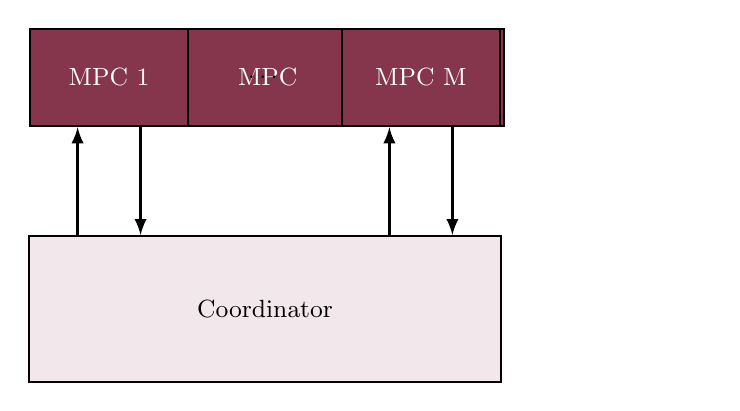
\begin{tikzpicture}[font=\small,thick,node distance=3*0.6180cm and 0.6180cm,every node/.style=rectangle,
        mpcSmall/.style={fill=mpc_agent, minimum height=0.6180*2cm, minimum width=2cm,text=white},
        coordinator/.style={fill=mpc_coordinator, minimum height=0.6180*3cm, minimum width=6cm},
        ]

        \visible<1>{
          % \node[ mpcSmall,fill=none] (block1) {\small MPC 1};
          \node[mpcSmall, draw, minimum width=6cm,right=-1cm] (mult) {\small MPC};
          \node[mpcSmall, fill=none, right=of mult,] (blockM) {\small MPC M};
        }
        \visible<2->{
          \node[draw, mpcSmall] (block1) {\small MPC 1};
          \node[fill=none, draw=none, right=of block1,] (mult) {\bf $\dots$};
          \node[draw, mpcSmall, fill=mpc_agent, right=of mult,] (blockM) {\small MPC M};
        }
        \onslide<3->{\node[draw, coordinator, below=of mult,] (coordinator) {Coordinator};}

        \onslide<4->{
          \draw[-latex,line width=1pt] (block1.south)+(0.4,.0) -- ( coordinator.north -| {$(block1.south)+(0.4,.0)$}) node [right,midway] {};
          \draw[latex-,line width=1pt] (block1.south)+(-0.4,0) -- (  coordinator.north -| {$(block1.south)+(-0.4,0)$}) node [left,midway] {};
          \draw[-latex,line width=1pt] (blockM.south)+(0.4,.0) -- ( coordinator.north -| {$(blockM.south)+(0.4,.0)$}) node [right,midway] {};
          \draw[latex-,line width=1pt] (blockM.south)+(-0.4,0) -- (  coordinator.north -| {$(blockM.south)+(-0.4,0)$}) node [left,midway] {};
        }
      \end{tikzpicture}
    \end{figure}
  \end{minipage}
  \hfill
  \begin{minipage}[c]{.5\linewidth}
    \begin{itemize}[<+(2)->]
      \item Coordinator $\to$ Hierarchical
      \item Bidirectional
      \item No delay $\to$ Synchronous
    \end{itemize}
    \vspace{.5cm}
    \begin{itemize}[<+(2)->]
      \item Agents solve local problems\tikzmark{a}
      \item Variables are updated
    \end{itemize}
    \onslide<+(2)->{
      \begin{tikzpicture}[overlay, remember picture,decoration={brace,amplitude=2pt}]
        \draw[decorate,thick] (a.north east) --+ (0,-1) node[midway, right=0.1cm,text=black,text width = 2in] {Until\\ Convergence};
      \end{tikzpicture}%
    }
    \centering
  \end{minipage}
\end{frame}

\begin{frame}{Distributed Model Predictive Control}
  Negotiation works if agents comply.\\\pause
  But what if some agents are ill-intentioned and attack the system?\\~\\\pause
  \begin{itemize}
    \item How can an agent attack?
    \item What are the consequences of an attack?
    \item Can we mitigate the effects?
  \end{itemize}
\centering
\onslide<+(1)->{~\\~\\Let's have a preview!}
\end{frame}

\begin{frame}{How can a non-cooperative agent attack?}{Literature}
\begin{minipage}[c]{.4\linewidth}
    \begin{figure}[H]
      \centering
      \begin{tikzpicture}[font=\small,thick,node distance=3*0.6180cm and 0.6180cm,every node/.style=rectangle,
        mpcSmall/.style={fill=mpc_agent, minimum height=0.6180*2cm, minimum width=2cm,text=white},
        coordinator/.style={fill=mpc_coordinator, minimum height=0.6180*3cm, minimum width=6cm},
        ]

        \only<1->{\node[draw, mpcSmall] (block1) {\small MPC 1};}
        \only<3->{\node[draw, mpcSmall,fill=white,path picture={\node at (path picture bounding box.center) {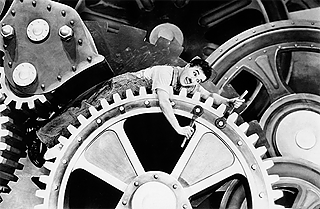
\includegraphics[height=1.5cm]{chaplin.png}};}] (block1) {\small };}
        \node[fill=none, draw=none, right=of block1,] (mult) {\bf $\dots$};
        \node[draw, mpcSmall, fill=mpc_agent, right=of mult] (blockM) {\small MPC M};
        \node[draw, coordinator, below=of mult,] (coordinator) {Coordinator};

        \draw[-latex,line width=1pt] (block1.south)+(0.4,.0) -- ( coordinator.north -| {$(block1.south)+(0.4,.0)$}) node [right,midway] {};
        \draw[latex-,line width=1pt] (block1.south)+(-0.4,0) -- (  coordinator.north -| {$(block1.south)+(-0.4,0)$}) node [left,midway] {};
        \draw[-latex,line width=1pt] (blockM.south)+(0.4,.0) -- ( coordinator.north -| {$(blockM.south)+(0.4,.0)$}) node [right,midway] {};
        \draw[latex-,line width=1pt] (blockM.south)+(-0.4,0) -- (  coordinator.north -| {$(blockM.south)+(-0.4,0)$}) node [left,midway] {};
      \end{tikzpicture}
    \end{figure}
  \end{minipage}
  \hfill
  \begin{minipage}[c]{.5\linewidth}
    \begin{itemize}[<+(1)->]
      \item \cite{VelardeEtAl2017a,ChanfreutEtAl2018} present attacks
            \begin{itemize}[<.(3)->]
              \item Fake objective function\tikzmark{a}
              \item Fake constraints
              \item Use different control
            \end{itemize}
    \end{itemize}
  \end{minipage}
  \onslide<+(3)->{
    \begin{tikzpicture}[overlay, remember picture,decoration={brace,amplitude=2pt}]
      \draw[decorate,thick] (a.north east) --+ (0,-1.) node[midway, right=0.1cm,text=black,text width = 2in] {Deception Attacks};
    \end{tikzpicture}%
  }

\end{frame}

\begin{frame}{How can a non-cooperative agent attack?}{Our approach}
\begin{minipage}[c]{.4\linewidth}
    \begin{figure}[H]
      \centering
      \begin{tikzpicture}[font=\small,thick,node distance=3*0.6180cm and 0.6180cm,every node/.style=rectangle,
        mpcSmall/.style={fill=mpc_agent, minimum height=0.6180*2cm, minimum width=2cm,text=white},
        coordinator/.style={fill=mpc_coordinator, minimum height=0.6180*3cm, minimum width=6cm},
        ]

        \node[draw, mpcSmall] (block1) {\small MPC 1};
        \node[fill=none, draw=none, right=of block1,] (mult) {\bf $\dots$};
        \node[draw, mpcSmall, fill=mpc_agent, right=of mult,] (blockM) {\small MPC M};
        \node[draw, coordinator, below=of mult,] (coordinator) {Coordinator};

        \draw[-latex,line width=1pt] (block1.south)+(0.4,.0) -- ( coordinator.north -| {$(block1.south)+(0.4,.0)$}) node [right,midway] {};
        \draw[latex-,line width=1pt] (block1.south)+(-0.4,0) -- (  coordinator.north -| {$(block1.south)+(-0.4,0)$}) node [midway] (lambda1) {};
        \draw[-latex,line width=1pt] (blockM.south)+(0.4,.0) -- ( coordinator.north -| {$(blockM.south)+(0.4,.0)$}) node [right,midway] {};
        \draw[latex-,line width=1pt] (blockM.south)+(-0.4,0) -- (  coordinator.north -| {$(blockM.south)+(-0.4,0)$}) node [left,midway] {};

        \only<3->{\node[draw,minimum height=0.3*2cm, minimum width=2cm,path picture={\node at (path picture bounding box.center) {
\includegraphics[height=1.5cm]{dick_dastardly.jpg}};}] at ($(lambda1)+(.4,0)$) {};}

      \end{tikzpicture}
    \end{figure}
  \end{minipage}
  \hfill
  \begin{minipage}[c]{.5\linewidth}
    \begin{itemize}[<+->]
      \item We are in coordinator's shoes
      \item What matters is the interface
            \begin{itemize}
              \item Attacker changes communication
                    \begin{itemize}
                      \item \alert<.(1)>{False Data Injection}
                    \end{itemize}
            \end{itemize}
    \end{itemize}
  \end{minipage}
\end{frame}


\begin{frame}{Consequence of an attack}
  \begin{overlayarea}{\textwidth}{.5\textwidth}
    \begin{itemize}[<+(1)->]
      \item Attack modifies optimization problem
            \begin{itemize}[<+(1)->]
              \item Optimum value is shifted
            \end{itemize}
    \end{itemize}
    \begin{minipage}[t]{.450\linewidth}
      \begin{figure}[h]
        \centering
        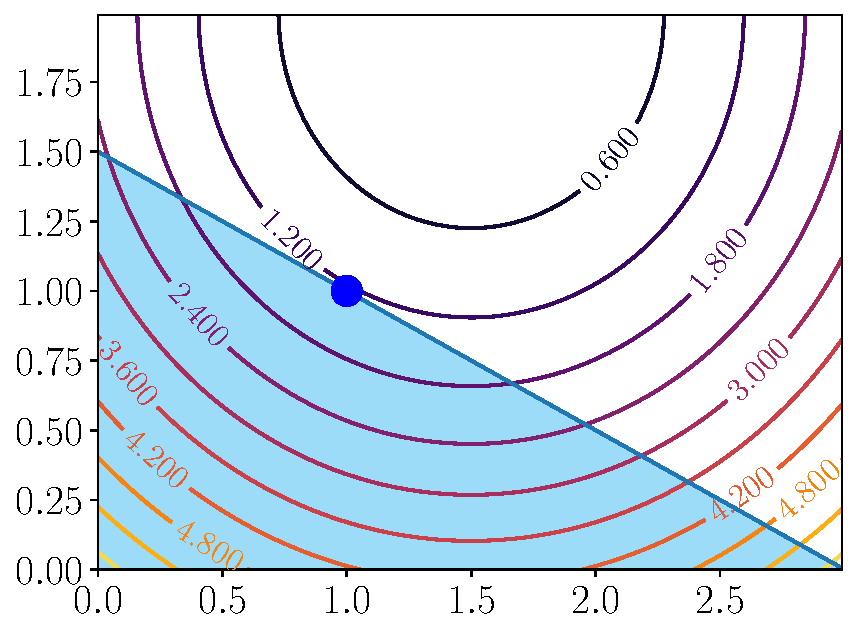
\includegraphics[width=\textwidth]{../img/resilient_eq/original-minimum.pdf}
        \caption*{Original minimum.}\label{fig:original_minimum}
      \end{figure}
    \end{minipage}
    \hfill
    \visible<+(-1)->{
      \begin{minipage}[t]{.45\linewidth}
        \begin{figure}[h]
          \centering
          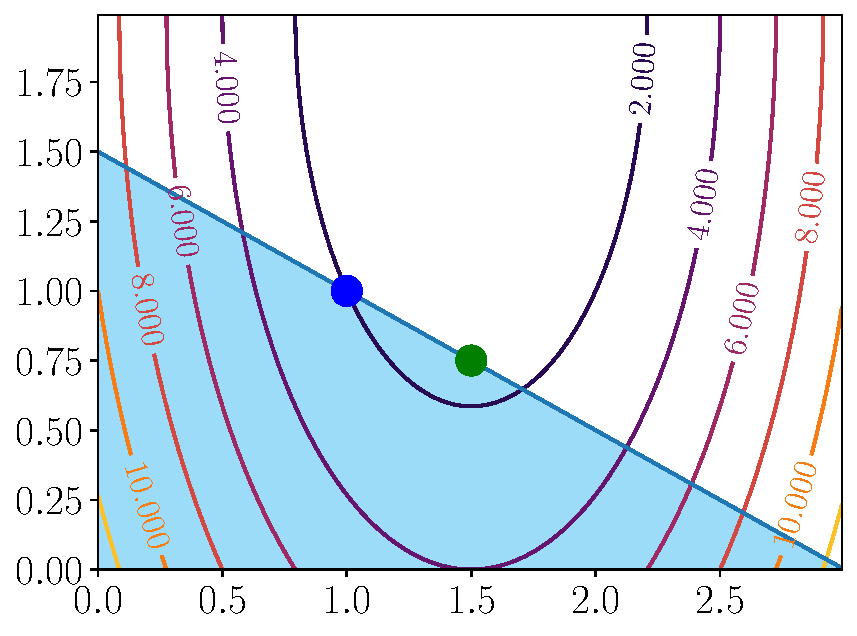
\includegraphics[width=\textwidth]{../img/resilient_eq/new-minimum-selfish.pdf}
          \caption*{Minimum after attack.}\label{fig:minimum_after_attack}
        \end{figure}
      \end{minipage}
    }
  \end{overlayarea}
\end{frame}

\begin{frame}{Mitigating the effects}
  \vspace{-1.cm}
  \begin{overlayarea}{\textwidth}{.4\textwidth}
    \begin{itemize}[<+(1)->]
      \item We can recover by
            \begin{itemize}[<+(1)->]
              \item Ignoring attacker
              \item Recuperating original behavior (at least trying)
            \end{itemize}
    \end{itemize}
      \only<2->{
        \vspace{-.4cm}
      \begin{minipage}[t]{.45\linewidth}
        \only<3->{
          \begin{figure}[h]
            \centering
            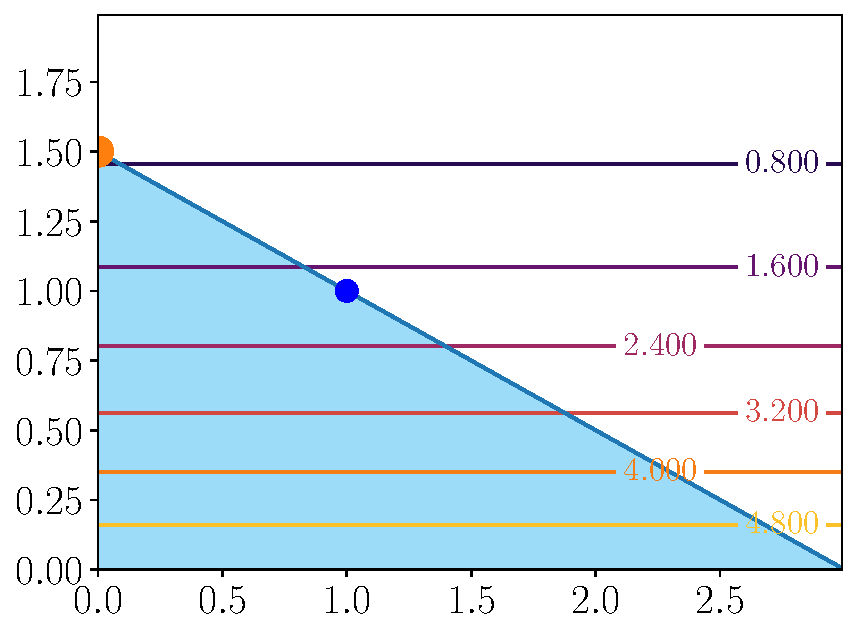
\includegraphics[width=\textwidth]{../img/resilient_eq/ignoreX.pdf}
            \caption*{Ignore attacker.}\label{fig:minimum_ignoring_attacker}
          \end{figure}
        }
      \end{minipage}
      \hfill
      \begin{minipage}[t]{.45\linewidth}
        \only<4->{
          \begin{figure}[h]
            \centering
            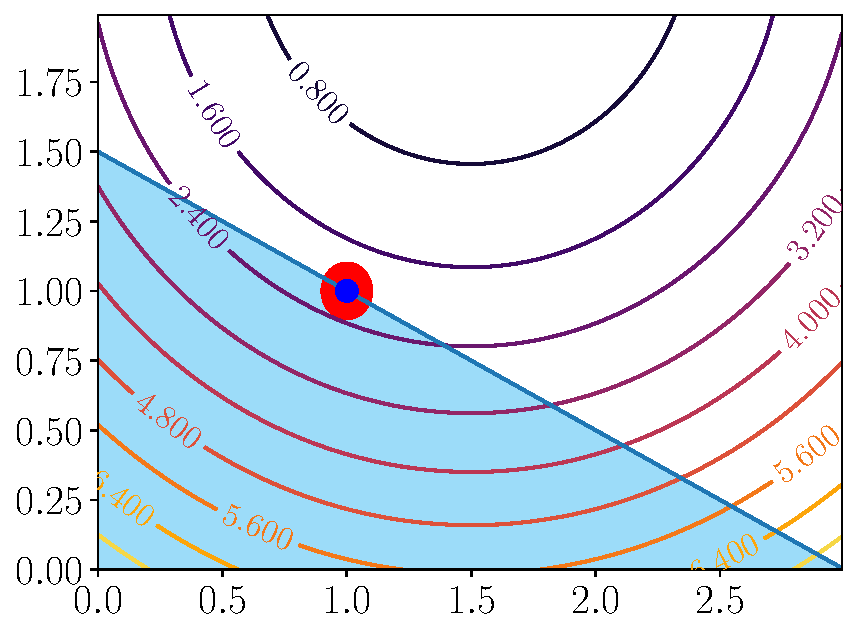
\includegraphics[width=\textwidth]{../img/resilient_eq/correctX.pdf}
            \caption*{\alert<5>{Recover original behavior}.}\label{fig:minimum_recovered}
          \end{figure}
        }
      \end{minipage}
    }
  \end{overlayarea}
\end{frame}

\begin{frame}{Classification of mitigation techniques}
  \begin{minipage}[t]{.45\linewidth}
    \onslide<1->{Passive (Robust)}
    \begin{itemize}
      \item<2-> 1 mode
    \end{itemize}
  \end{minipage}
  \hfill
  \begin{minipage}[t]{.45\linewidth}
    \onslide<1->{\alert<5>{Active (Resilient)}}
    \begin{itemize}
      \item<2-> 2 modes
            \begin{enumerate}
              \item<3-> Attack free
              \item<3-> When attack is detected
                    \begin{itemize}
                      \item<4-> Detection/Isolation
                      \item<4-> Mitigation
                    \end{itemize}
            \end{enumerate}
    \end{itemize}
  \end{minipage}
\end{frame}

\begin{frame}{State of art}{Security dMPC}
  \begin{table}[H]
    \resizebox{.9\textwidth}{!}{
      \begin{tabular}[h]{l!{\vrule}cc<{\onslide<5->}c<{\onslide<5->}c<{\onslide}}
        \toprule
        & Decomposition & Resilient/Robust & Detection & Mitigation\\
        \midrule
        {\cite{VelardeEtAl2017a}}\\ \cite{MaestreEtAl2021} & Dual &  Robust (Scenario) & NA & NA\\\\
        \cite{VelardeEtAl2017b} \\ \cite{VelardeEtAl2018} & Dual &  Robust (f-robust) & NA & NA\\\\
        {\cite{ChanfreutEtAl2018}} & Jacobi-Gauß &  -- & -- & --\\\\
        \cite{AnandutaEtAl2018}\\\cite{AnandutaEtAl2019}\\\cite{AnandutaEtAl2020} & Dual &  Resilient& Analyt./Learn. & Disconnect (Robustness)\\
        \\\midrule
        \visible<2->{
        \only<5->{\\[-\normalbaselineskip]\rowcolor{ietrRed!10}}\Large Our &\Large \alert<3->{Primal} & \Large \alert<4->{Resilient} & \Large Active Analyt./Learn. & \Large \alert<6->{Data reconstruction}}
        \\\bottomrule
      \end{tabular}
    }
  \end{table}
\end{frame}


% % % Structuring a talk is a difficult task and the following structure
% % % may not be suitable. Here are some rules that apply for this
% % % solution:

% % % - Exactly two or three sections (other than the summary).
% % % - At *most* three subsections per section.
% % % - Talk about 30s to 2min per frame. So there should be between about
% % % 15 and 30 frames, all told.

% % % - A conference audience is likely to know very little of what you
% % % are going to talk about. So *simplify*!
% % % - In a 20min talk, getting the main ideas across is hard
% % % enough. Leave out details, even if it means being less precise than
% % % you think necessary.
% % % - If you omit details that are vital to the proof/implementation,
% % % just say so once. Everybody will be happy with that.

\begin{frame}{Outline}
  % \tableofcontents
  \tableofcontents[subsectionstyle=hide/hide/hide,pausesections]
  % You might wish to add the option [pausesections]
  \begin{itemize}[<+(1)->]
    \item \encircle{1} and \encircle{2} yielded \cite{NogueiraEtAl2021} (SysTol'21)
    \item \encircle{3} yielded \cite{NogueiraEtAl2022} (NecSys'22)\tikzmark{a}
  \end{itemize}
  \script<1->{To respond this this presentation is divided into 3 parts.}
  \script<1->{First we present the decomposition and its vulnerabilites, }
  \script<2->{We propose a resilient method for two kind of systems with increasing complexities.}

  \onslide<.(2)->{\begin{tikzpicture}[overlay, remember picture,node distance=0.1pt and 0.025cm]
    \draw[thick,->] ($(a.center) +( 1,0 ) $) --+ (1,.5) node[] (image) {};
    \node[right=.5cm,inner sep=1pt] (simon) at (8,1.5)  {
      \includegraphics[width=2cm]{simon.png}
    };
    \node[below=of simon,align=center] {Simon Leglaive\\AIMAC Team};
  \end{tikzpicture}%
  }

\end{frame}

\section[Vulnerabilities in dMPC based on Primal decomposition]{Vulnerabilities in distributed MPC based on Primal Decomposition}

\subsection{What is the Primal Decomposition?}

\begin{frame}{Primal Decomposition}{or Quantity Decomposition | or Resource Allocation}
  \centering
  \begin{minipage}{.45\linewidth}
    \begin{figure}
      \centering
      \scalebox{.55}{
        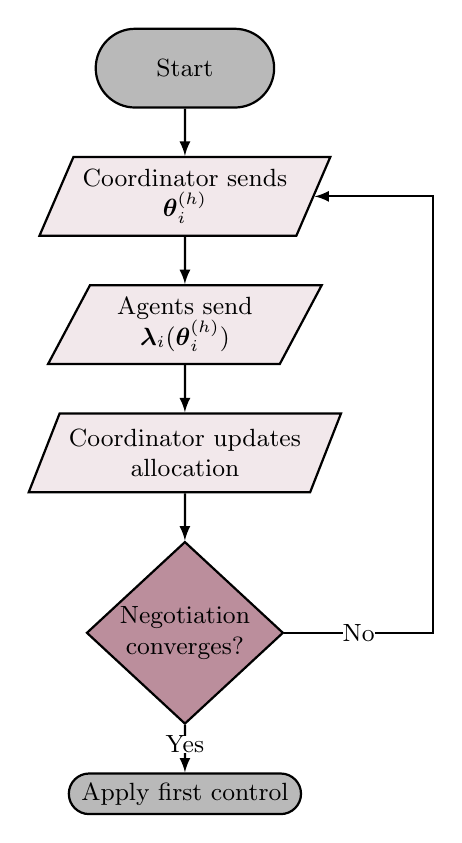
\begin{tikzpicture}[font=\small,thick,node distance=.6cm and 6cm,
          action/.style={draw, trapezium, trapezium left angle = 65, trapezium right angle = 115, trapezium stretches, align=center, fill=supelecRed!10, minimum width=3.5cm, minimum height=1cm,},
          terminal/.style={draw, rounded rectangle, fill=gray!90!black!50, minimum height=1cm, minimum width=2.5cm,},
          condition/.style={draw, diamond, fill=supelecRed!50,minimum width=2.5cm,align=center, inner sep=0},
          selected/.style={fill=supelecRed!90, text=white}
          ]

          \node[terminal, alt=<{2}>{selected}] (block1) {Start};

          \node[action, alt=<{3}>{selected},below=of block1,] (block7) { Coordinator sends \\$\vec{\theta}_i^{(h)}$};

          \node[action, alt=<{4}>{selected}, below=of block7,] (block8) { Agents send \\$\vec{\lambda}_i(\vec{\theta}_{i}^{(h)})$};

          \node[action, alt=<{5}>{selected}, below=of block8,
          ] (block9) { Coordinator updates \\allocation};

          \node[condition, alt=<{6}>{selected}, below=of block9] (block10) { Negotiation\\ converges?};

          \node[draw,
          rounded rectangle,
          below=of block10,
          fill=gray!90!black!50,
          alt=<{7}>{selected},
          ] (block11) { Apply first control};

          \draw[-latex] (block7) edge (block8) (block1) edge (block7) (block8) edge (block9) (block9) edge (block10);

          \draw[-latex] (block10) -- (block11) node[pos=0.4,fill=white,inner sep=0]{Yes};

          \draw[-latex] (block10) -| ($(block7.east) + (1.5cm,0)$)
          node[pos=0.25,fill=white,inner sep=0]{No} -- (block7.east);

        \end{tikzpicture}
      }
      % \caption{Quantity decomposition based DMPC}\label{fig:quantityDecompDMPC}
    \end{figure}
  \end{minipage}
  \only<2->{\begin{minipage}{.45\linewidth}
      \begin{figure}
        \centering
        \begin{tikzpicture}[balloon/.style={
            line width=1pt, draw, ellipse callout,
            align=center, inner sep=.1cm}]
          \node (image) {
            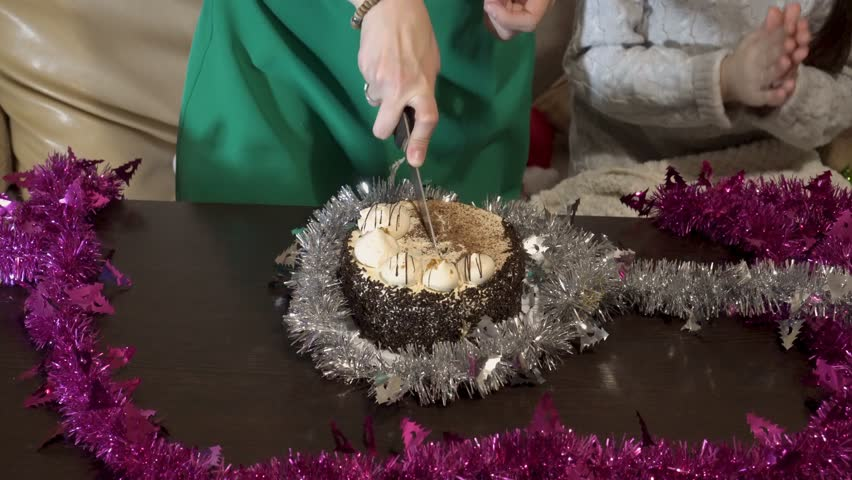
\includegraphics[width=\textwidth,trim=2cm 2 20 4,clip]{cut-cake.jpg}
          };
          \visible<3->{\node at ($(image.center)+(-0.0cm,3.0cm)$) {\alert<3>{Allocation $\vec{\theta}_{i}$}};}
          \visible<4->{\node at ($(image.center)+(-0.0cm,2.5cm)$) {\alert<4>{Dissatisfaction $\vec{\lambda}_{i}$}};}
          \visible<5->{\node at ($(image.center)+(-0.0cm,-2.5cm)$) {\alert<5>{Update $\vec{\theta}_{i}^{+}=f_{i}(\vec{\theta}_{i},\vec{\lambda}_{i})$}};}

          \visible<3>{\node[balloon,fill=blue!50, callout relative pointer={(0,1)}] at ($(image.center)+(-.5cm,0.8cm)$) {Is it ok?};}
          \visible<4>{\node[balloon,fill=green!50, callout relative pointer={(-1,1)}] at ($(image.center)+(-1.5cm,1.0cm)$) {I want more!};}
          \visible<4>{\node[balloon,fill=red!50, callout relative pointer={(1,1)}] at ($(image.center)+(1.5cm,1.0cm)$) {I want more!};}
          \visible<5>{\node[balloon,fill=blue!50, callout relative pointer={(0,1)}] at ($(image.center)+(-.5cm,0.8cm)$) {And like this?};}
          \visible<6>{\node[balloon,fill=blue!50, callout relative pointer={(0,1)}] at ($(image.center)+(-.5cm,0.5cm)$) {Guys,\\ let's compromise ...};}
        \end{tikzpicture}
      \end{figure}
    \end{minipage}}
  \script<1->{In a flowchart for a quantity decomposition based DMPC,}
  \script<3->{the coordinator sends the allocation theta, }
  \script<4->{the agents send the dual variable lambda, }
  \script<5->{the coordinator updates the allocation. }
  \script<6->{If negotiation converges, }
  \script<7->{then the negotiation ends and each agent applies the first element of the control found}
\end{frame}

\begin{frame}{Primal Decomposition }{In detail}
  \begin{minipage}[c]{.45\linewidth}
    \begin{itemize}
      \item<2-> Objective is sum of local ones
      \item<3-> Constraints couple variables
    \end{itemize}
  \end{minipage}
  \hfill
  \begin{minipage}[c]{.45\linewidth}
    \onslide<1-4>{
      \begin{equation*}
        \begin{matrix}
          \minimize\limits_{\vec{u}_{1},\dots,\vec{u}_{M}} & \alert<2>{\sum\limits_{i\in\set{M}}J_{i}(\vec{x}_{i},\vec{u}_{i})}\\
          \alert<3>{\mathrm{s.t.}} &\alert<3>{\sum\limits_{i\in\set{M}}\vec{h}_{i}(\vec{x}_{i},\vec{u}_{i})\preceq \vec{u}_{\text{total}}}
        \end{matrix}
      \end{equation*}
    }
  \end{minipage}

  \begin{minipage}[c]{.5\linewidth}
    \begin{enumerate}
      \item<5-> Allocate $\thetai$ for each agent
      \item<6-> They solve local problems and
      \item<7-> Send dual variable $\lambdai$
      \item<8-> Allocation is updated \onslide<9->{\\(respecting global constraint)}
    \end{enumerate}
  \end{minipage}
  \hfill
  \begin{minipage}[c]{.45\linewidth}
    \onslide<4->{
      \begin{equation*}
        \begin{matrix}
          \minimize\limits_{\vec{u}_{i}} & J_{i}(\vec{x}_{i},\vec{u}_{i})\\
          {\mathrm{s.~ t.}} &{\vec{h}_{i}(\vec{x}_{i},\vec{u}_{i})\preceq \alert<5>{\vec{\theta}_{i}}} \onslide<7->{\alert<7>{: \vec{\lambda}_{i}}}
        \end{matrix}
      \end{equation*}
    }
    \onslide<8->{
      \begin{equation*}
        \vec{\theta}[k]\pplusone=\onslide<9->{\Proj^{\tikzmark{sets}\set{S}}(}\vec{\theta}[k]\p+\rho\p\vec{\lambda}[k]\p\onslide<9->{)}
      \end{equation*}
    }
  \end{minipage}
  \onslide<4>{
    \begin{tikzpicture}[overlay, remember picture]
      \draw[->] (-2.,2) -- +(0,-.5) node[midway,right=0.25cm] {For each $i\in\set{M}$};
    \end{tikzpicture}
  }
\end{frame}

\begin{frame}{Example}
  \centering
  Until everybody is equally dissatisfied
  % \centering
  \vspace{1cm}

  \begin{minipage}{0.45\textwidth}
    \begin{figure}
      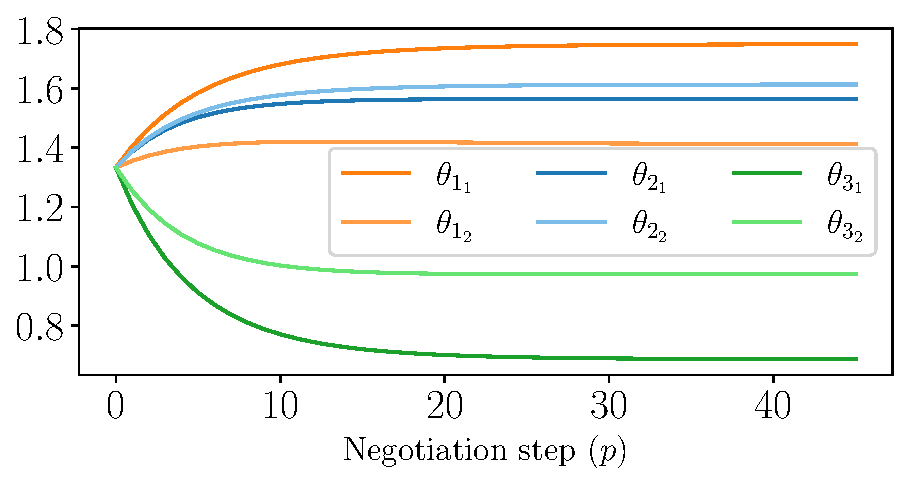
\includegraphics[width=\textwidth]{../img/example_primal_decomposition/example_theta.pdf}
    \end{figure}
  \end{minipage}
  \hfill
  \begin{minipage}{0.45\textwidth}
    \begin{figure}
      \centering
      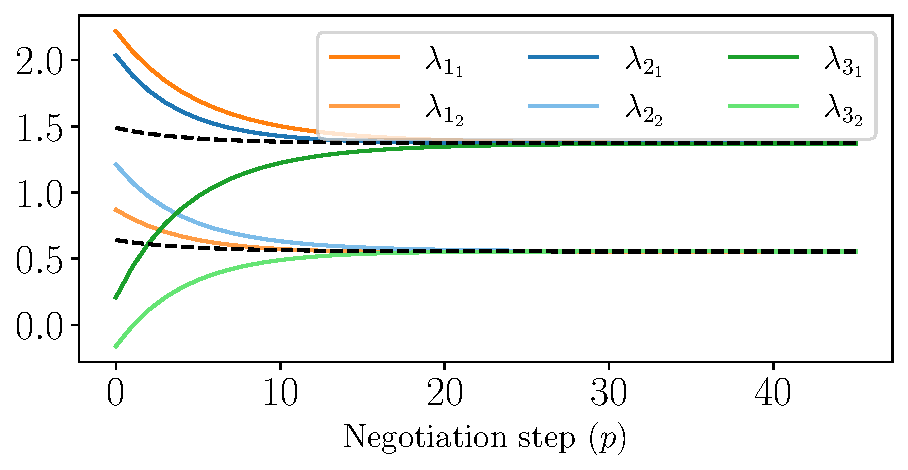
\includegraphics[width=\textwidth]{../img/example_primal_decomposition/example_lambda.pdf}
    \end{figure}
  \end{minipage}
\end{frame}

% \begin{frame}{Distributed Model Predictive Control}{In our case}
%   \begin{minipage}{0.45\textwidth}
%     \begin{assumptions}
%       \begin{itemize}[<+(1)->]
%         \item Sum of \alert<2>{Quadratic} objectives
%         \item Linear subsystems
%         \item Coupled by the inputs
%       \end{itemize}
%     \end{assumptions}
%   \end{minipage}
%   \quad
%   \begin{minipage}{0.45\textwidth}
%     \onslide<5-6>{
%       \begin{equation*}
%         \begin{matrix}
%           \small
%           \minimize\limits_{\vec{U}_{1}[k],\dots, \vec{U}_{M}[k]} &
%                                                                     \sum\limits_{i\in\set{M}}\frac{1}{2}\norm{\vec{U}_{i}[k]}^{2}_{H_{i}} + {\vec{f}_{i}[k]}^{T}\vec{U}_{i}[k]&\\
%           \mathrm{subject~ to} & \sum\limits_{i\in\set{M}}\bar{\Gamma}_{i}\vec{U}_{i}[k] \preceq {\vec{U}}_{\text{max}}
%         \end{matrix}
%       \end{equation*}
%     }
%   \end{minipage}

%   \onslide<8>{
%     \begin{tikzpicture}[overlay, remember picture]
%       \usebeamercolor{framesubtitle}
%       \draw[bg,fill=bg] (6.25,1.5) rectangle +(7.,-2.6);
%     \end{tikzpicture}
%   }
%   \begin{minipage}{0.45\textwidth}
%     \begin{itemize}[<+(2)->]
%       \item Local problems
%       \item Update function
%     \end{itemize}
%   \end{minipage}
%   \quad
%   \begin{minipage}{0.45\textwidth}
%     \onslide<6->{
%       \begin{equation*}
%         \begin{matrix}
%           \small
%           \minimize\limits_{\vec{U}_{i}[k]}&\frac{1}{2}\norm{\vec{U}_{1}[k]}^{2}_{H_{i}} + {\vec{f}_{i}[k]}^{T}\vec{U}_{i}[k]\\
%           \mathrm{subject~ to} & \bar{\Gamma}_{i}\vec{U}_{i}[k] \preceq \tikzmark{theta1}{\mpcvec{\theta}[i][k]}{{:\mpcvec{\lambda}[i][k]}}

%         \end{matrix}
%       \end{equation*}
%     }
%     \onslide<7->{
%       \begin{equation*}
%         \vec{\theta}[k]\pplusone=\Proj^{\tikzmark{sets}\set{S}}(\vec{\theta}[k]\p+\rho\p\vec{\lambda}[k]\p)
%       \end{equation*}
%     }
%   \end{minipage}
%   \onslide<6>{
%     \begin{tikzpicture}[overlay, remember picture]
%       \draw[->] (-2.,2.) -- +(0,-.5) node[midway,right=0.25cm] {For each $i\in\set{M}$};
%     \end{tikzpicture}
%   }

%   \script<1->{An example of decomposition method is the Quantity decomposition where a semi-decomposable problem with a global coupling constraints can be decomposed into }
%   \script<2->{multiple sub-problems, which can be solved in parallel, and a master problem which corresponds to the initial problem. \\ Those coupling constraints are replaced by local constraints with an allocation theta i. }
%   \script<3->{The allocation for each sub-problem is updated by a projected subgradient method solving the master problem, thus the original problem. The subgradient used in this method is the dual variable associated to the coupling constraints}
%   \script<4->{We can represent the sub-problems as agents and the master problem as a coordinator. The coordinator sends the allocations for each agent, which responds with a dual variable. }
% \end{frame}

\subsection{How can an agent attack?}


\begin{frame}{How can a non-cooperative agent attack?}{Our approach}
    \begin{minipage}[c]{.35\linewidth}
      \scalebox{.8}{
        \begin{tikzpicture}[font=\small,thick,node distance=3*0.6180cm and 1.cm,every node/.style=rectangle,
          mpcSmall/.style={fill=mpc_agent, minimum height=0.6180*2cm, minimum width=2cm,text=white},
          coordinator/.style={fill=mpc_coordinator, minimum height=0.6180*3cm, minimum width=7cm},
          ]

          \node[draw, mpcSmall] (block1) {\small MPC 1};
          \node[fill=none, draw=none, right=of block1,] (mult) {\bf $\dots$};
          \node[draw, mpcSmall, fill=mpc_agent, right=of mult,] (blockM) {\small MPC M};
          \node[draw, coordinator, below=of mult,] (coordinator) {Coordinator};

          \only<-3>{\draw[-latex,line width=1pt] (block1.south)+(0.4,.0) -- ( coordinator.north -| {$(block1.south)+(0.4,.0)$}) node (lambda1) [right,midway] {$\alert<3>{\lambda_{1}}$};}
          \only<4->{\draw[-latex,line width=1pt] (block1.south)+(0.4,.0) -- ( coordinator.north -| {$(block1.south)+(0.4,.0)$}) node (lambda1) [right,midway] {$\alert<4->{\tilde{\lambda}_{1}}$};}
          % \only<3->{\node[draw, mpcSmall,] (block1) {};}
          \only<3->{\node[draw,minimum height=0.6180*1.75cm, minimum width=1.75cm,path picture={\node at (path picture bounding box.center) {
\includegraphics[height=1.5cm]{dick_dastardly.jpg}};}] at ($(lambda1)+(1.2,0)$) {};}

          \draw[latex-,line width=1pt] (block1.south)+(-0.4,0) -- (  coordinator.north -| {$(block1.south)+(-0.4,0)$}) node [left,midway] {$\theta_{1}$};
          \draw[-latex,line width=1pt] (blockM.south)+(0.4,.0) -- ( coordinator.north -| {$(blockM.south)+(0.4,.0)$}) node [right,midway] {$\lambda_{M}$};
          \draw[latex-,line width=1pt] (blockM.south)+(-0.4,0) -- (  coordinator.north -| {$(blockM.south)+(-0.4,0)$}) node [left,midway] {$\theta_{M}$};
        \end{tikzpicture}
      }
    \end{minipage}
    \hfill
    \begin{minipage}[c]{.5\linewidth}
      \begin{overlayarea}{\textwidth}{0.4\textwidth}
      \begin{itemize}
        \item<1-> $\vec{\lambda}_{i}$ is the only interface
        \item<2-> $\vec{\lambda}_{i}$ depends on local parameters
        \item<3-> Malicious agent modifies $\vec{\lambda}_{i}$
      \end{itemize}
      \centering
      \only<4->{$\tilde{\vec{\lambda}}_{i}=\gamma_{i}(\vec{\lambda}_{i})$\\}
    \end{overlayarea}
    \end{minipage}
  \script<2->{How can an agent attack the system? Its only interface with the coordination is lambda}
  \script<3->{so we suppose it attacks by sending a different $lambda_i$, modified by a function $gamma_i$ of $lambda_i$ }
\end{frame}

\begin{frame}{How does an agent lie?}{Liar, Liar, Pants of fire}
  \begin{minipage}[c]{.5\linewidth}
    \begin{itemize}[<+(1)->]
      \item $\lambda\ge 0$ means dissatisfaction
      \item $\lambda=0$ means complete satisfaction
    \end{itemize}
    \pause
    \begin{assumptions}
      \begin{itemize}[<+(1)->]
        \item Same attack during negotiation
        \item Attacker satisfied only if it really is
              \begin{itemize}
                \item $\gamma(\lambda)=0\rightarrow \lambda=0$
              \end{itemize}
        \item $\lambdaicheat=\Tik\lambdai$
      \end{itemize}
    \end{assumptions}
    \begin{itemize}[<+(1)->]
      \item Attack is invertible \onslide<+(1)->{$\to \exists \Tik^{-1}$}
    \end{itemize}
  \end{minipage}
  \hfill
  \begin{minipage}[c]{.4\linewidth}
    \definecolor{mycolor1}{rgb}{0.47000,0.12000,0.22000}%
    \onslide<11->{
      \begin{tikzpicture}[domain=0:2]
        % \draw[very thin,color=gray] (-0.1,-1.1) grid (3.9,3.9);
        \draw[-latex] (-0.2,0) -- (4.2,0) node[below] {$\lambda$};
        \draw[-latex] (0,-0.2) -- (0,4.2) node[left] {$\gamma(\lambda)$};
        \node[below left] (0,0) {0};
        \only<12>{\draw[red] (0,0) circle (0.1);}

        \only<11->{\draw[color=gray,dashed,domain=0:4] plot (\x,\x);}

        % \x r means to convert '\x' from degrees to _r_adians:
        % \only<7-8>{\draw[color=mycolor1,domain=0:.85] plot (\x,{exp(1.7*\x)-1+0.2*sin(25*\x r)}) node[right] {};}
        \only<8>{\node[red,draw,solid,cross out,inner sep=.25cm,thick] at (0.5,1.5) {};}
        \only<9>{\draw[color=orange,domain=0:1.5] plot (\x,{exp(\x)-1}) node[right] {$\mathrm e^\lambda-1$};}
        \only<12->{\draw[color=blue,domain=0:1.25] plot (\x,3*\x) node[above,xshift=.9cm] {$a\lambda\text{, }a>1$} ;}
      \end{tikzpicture}
    }
  \end{minipage}
\end{frame}

\subsection{Consequences}

\begin{frame}{Example}
  \centering
  \begin{minipage}[c]{.4\linewidth}
    \begin{figure}[!t]
      \centering
      \begin{tikzpicture}
        \visible<3->{\node (0,0){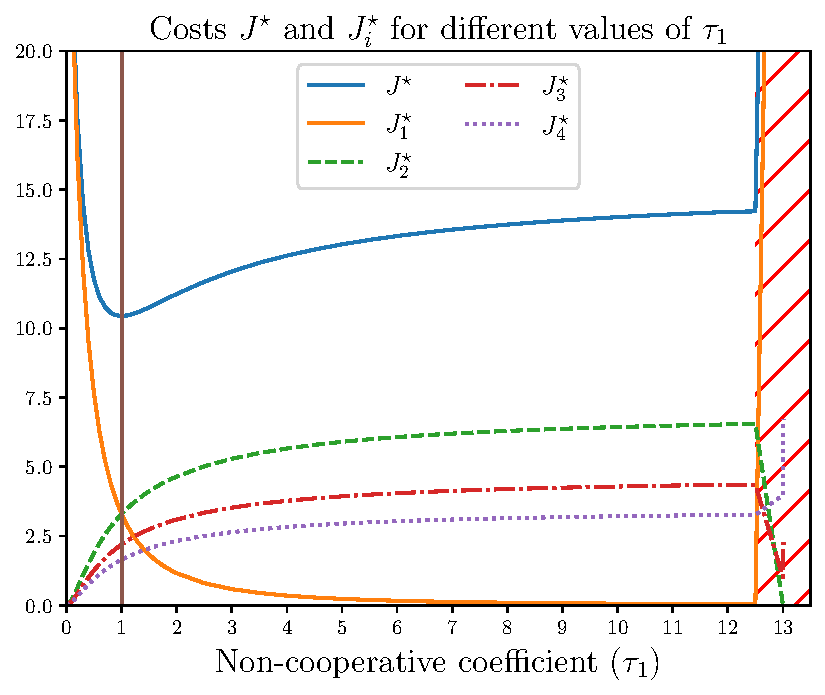
\includegraphics[width=\textwidth]{changeOfJ.pdf}};}
        \usebeamercolor{alerted text}
        \draw<5>[rounded corners,fg,thick] (-2.1,2.) rectangle +(.5,-4);
        \draw<7>[rounded corners,fg,thick] (1.9,2.) rectangle +(.75,-4);
      \end{tikzpicture}
    \end{figure}
  \end{minipage}
  \hfill
  \begin{minipage}[c]{.5\linewidth}
    \onslide<2->{
      \begin{exampleblock}{4 distinct agents}
        \begin{itemize}
          \item Agent 1 is non-cooperative\\
          \item It uses $\tilde{\vec{\lambda}}_{1}=\gamma_{1}(\vec{\lambda}_{1})=\tau_{1}I\vec{\lambda}_{1}$
        \end{itemize}
      \end{exampleblock}
    }
    \begin{itemize}[<+(3)->]
      \item We can observe 3 things
            \begin{itemize}[<+(3)->]
              \item Global minimum when $\tau_{1}=1$
              \item Agent 1 benefits if $\tau_{1}$ increases (inverse otherwise)
              \item All collapses if too greedy
            \end{itemize}
    \end{itemize}
  \end{minipage}
  \script<1->{We give an example of 4 agents negotiating }
  \script<2->{Agent 1 is non-cooperative\\ }
  \script<3->{It uses a linear cheating function gamma tau times identity times the original lambda i\\ }
  \script<3->{In the figure we can see the cost functions for each agent, we see that agent 1 cost decreases if we increase tau, but the overall cost is increased, The minimum value of the global cost is when \\ }
  \script<4->{tau is equal to one. If tau is close to zero it increases its cost and if tau is too high\\ }
  \script<5->{it can turn the negotiation unstable \\ }
\end{frame}

\begin{frame}{}
  \begin{itemize}[<+(1)->]
    \item But can we mitigate these effects?
    \item Yes! \pause (At least in some cases)
  \end{itemize}

\end{frame}

\section{Resilient Primal Decomposition-based dMPC for deprived systems}
\subsection{Analyzing deprived systems}

\begin{frame}{What are deprived systems?}{}
  \centering
  \onslide<+(1)->{Systems whose optimal solution has all constraints active}

  % \begin{overlayarea}{\textwidth}{.5\textwidth}
  \begin{minipage}[t]{.55\linewidth}
    \begin{itemize}[<+(2)->]
      \item Unconstrained Solution $\optuncUik$
      \item $\bar{\Gamma}_{i}\optuncUik \succeq\thetaik$ $\to$ Scarce resources
            \begin{itemize}
              \item Solution projected onto boundary
              \item Same as with equality constraints\footnotemark

            \end{itemize}
    \end{itemize}

  \end{minipage}
  \quad
  \begin{minipage}[t]{.35\linewidth}
    \begin{figure}[h]
      \centering
      \visible<3->{
        \begin{tikzpicture}
          \visible<2-5>{\node at (0,0) {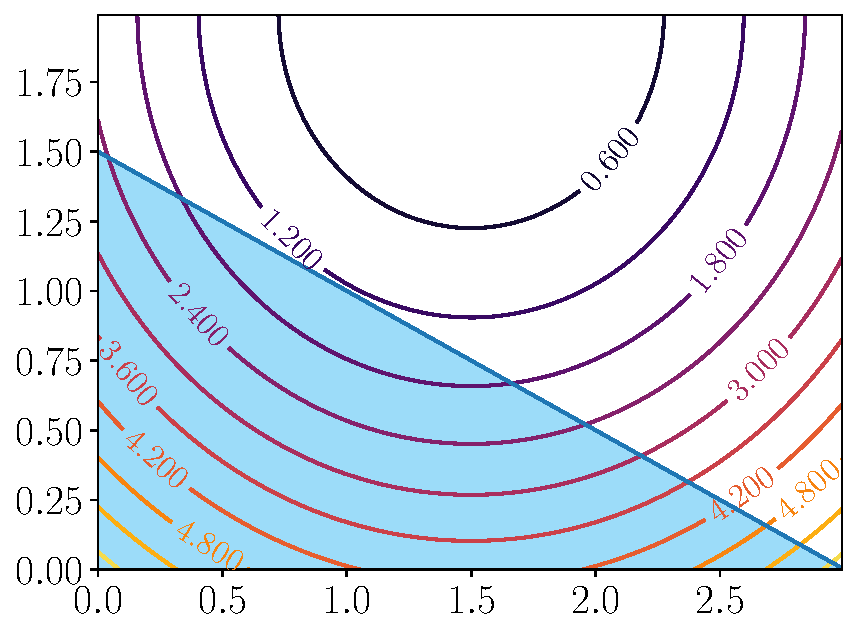
\includegraphics[width=1.\textwidth]{../img/resilient_eq/original-minimum_no_dots.pdf}};}
          \visible<6->{\node at (0,0) {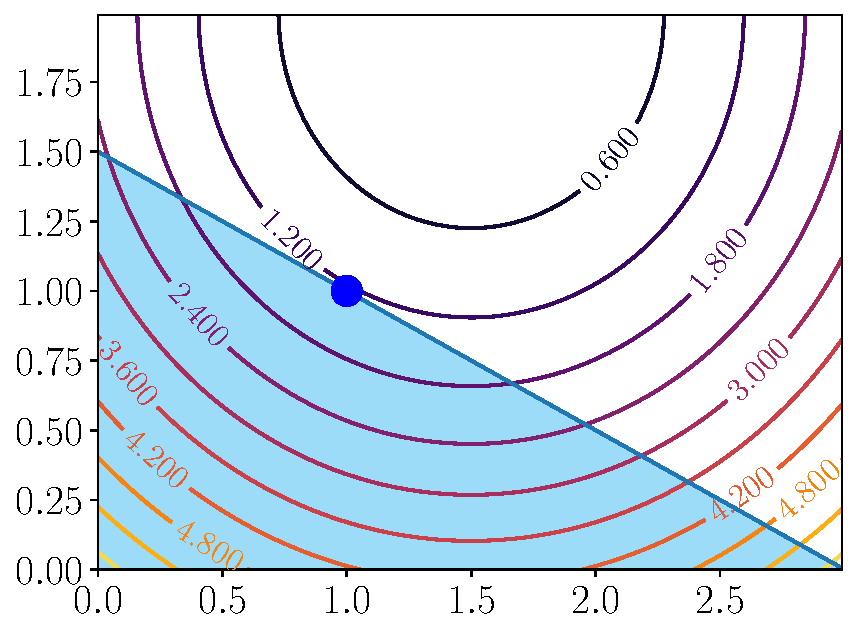
\includegraphics[width=1.\textwidth]{../img/resilient_eq/original-minimum.pdf}};}
          \visible<4->{\draw[fill] (0.2,1.2) circle (.05) node[below] {$\optuncUik$};}
          \visible<6->{\draw[fill,mpc_green!55!black] (-0.375,0.125) circle (0.075)  node[below=0.1cm,mpc_green!55!black] {$U_{i}^{\star}[k]$};}
        \end{tikzpicture}
      }
    \end{figure}
  \end{minipage}

  \centering
  \begin{minipage}[c]{.45\linewidth}
    \scriptsize
    \onslide<3->{
      \begin{equation*}
        \begin{matrix}
          \alert<4>{\minimize\limits_{\vec{U}_{i}[k]}}&\alert<4>{\frac{1}{2}\norm{\vec{U}_{i}[k]}^{2}_{H_{i}} + {\vec{f}_{i}[k]}^{T}\vec{U}_{i}[k]}\\
          \mathrm{subject~ to} & \bar{\Gamma}_{i}\vec{U}_{i}[k]  \preceq\thetaik:\lambdaik
        \end{matrix}
      \end{equation*}
    }
  \end{minipage}
  \hfill
  \onslide<7->{$\to$}
  \hfill
  \begin{minipage}[c]{.45\linewidth}
    \scriptsize
    \onslide<7->{
      \begin{equation*}
        \begin{matrix}
          \minimize\limits_{\vec{U}_{i}[k]}&\frac{1}{2}\norm{\vec{U}_{i}[k]}^{2}_{H_{i}} + {\vec{f}_{i}[k]}^{T}\vec{U}_{i}[k]\\
          \mathrm{subject~ to} & \bar{\Gamma}_{i}\vec{U}_{i}[k] = \thetaik:\lambdaik
        \end{matrix}
      \end{equation*}
    }
  \end{minipage}

  \onslide<7->{\footnotetext<7->{If system can have all constraints active simultaneously \hypertarget<7->{analysis_deprived_systems}{}
      \hyperlink<7->{condition_transform_equality}{\beamergotobutton{see here}} }}
  % \end{overlayarea}
\end{frame}

% \begin{frame}{Deprived Systems}{But why?}
%   \centering
%   \begin{minipage}[t]{.45\linewidth}
%     \begin{itemize}
%       \item<+(1)-> No Scarcity
%             \begin{itemize}[<+(1)->]
%               \item[$\to$] All constraints satisfied
%               \item[$\to$] No coordination needed
%               \item[$\to$] No incentive to cheat
%             \end{itemize}
%     \end{itemize}
%   \end{minipage}
%   \hfill
%   \begin{minipage}[t]{.45\linewidth}
%     \begin{itemize}[<+(1)->]
%       \item Scarcity
%             \begin{itemize}[<+(1)->]
%               \item[$\to$] Competition
%               \item[$\to$] Consensus/Compromise
%               \item[$\to$] Agents may cheat {\color{red}\faUserSecret}
%             \end{itemize}
%     \end{itemize}
%   \end{minipage}
% \end{frame}

\begin{frame}{Deprived Systems}{Analysis}
  \begin{minipage}[t]{.45\textwidth}
    \begin{assumptions}
      \begin{itemize}[<+(1)->]
        \item Quadratic local problems
        \item Scarcity
      \end{itemize}
    \end{assumptions}
  \end{minipage}
  \hfill
  \begin{minipage}[t]{0.45\textwidth}
    \centering
    \onslide<+(1)->{
      \begin{equation*}
        \small
        \begin{matrix}
          {\minimize\limits_{\vec{U}_{i}[k]}}&{\frac{1}{2}\norm{\vec{U}_{i}[k]}^{2}_{H_{i}} + {\vec{f}_{i}[k]}^{T}\vec{U}_{i}[k]}\\
          \mathrm{subject~ to} & \bar{\Gamma}_{i}\vec{U}_{i}[k] = \thetaik:\lambdaik \\
                                             &\\
        \end{matrix}
      \end{equation*}
    }
  \end{minipage}

  \begin{itemize}[<+(1)->]
    \item Solution is analytical and affine
          \onslide<+(1)->{
          \begin{equation*}
            \lambdaik=-\alert<.(2)>{\Plin}\thetaik-\alert<.(3)>{\sik}
          \end{equation*}
          }
  \end{itemize}

  \vspace{-.5cm}
  \hfill
  \begin{minipage}[t]{.45\linewidth}
    \begin{itemize}[<+(1)->]
      \item $\Plin$ is time invariant \tikzmark{a}
      \item $\sik$ is time variant
    \end{itemize}
  \end{minipage}
  \onslide<+(1)->{
    \begin{tikzpicture}[overlay, remember picture,decoration={brace,amplitude=2pt}]
      \draw[thick,decorate] ($(a.north east) +(-4,-1)$) --+ (0,1) node[midway, left=0.1cm,text=black] {(local parameters unknown by coordinator)};
    \end{tikzpicture}%
  }
\end{frame}

\begin{frame}{Deprived Systems}{Under attack!}
  \begin{minipage}[t]{.45\linewidth}
    \begin{itemize}[<+->]
      \item Normal behavior
            \begin{itemize}
              \item Affine solution
                    \begin{equation*}
                      \lambdaik=-\Plin\thetaik-\sik
                    \end{equation*}
            \end{itemize}
    \end{itemize}
  \end{minipage}
  \hfill
  \begin{minipage}[t]{.45\linewidth}
    \begin{itemize}
      \item<+-> Under attack \onslide<+->{$\to$ $\lambdaicheat=\Tik\lambdai$}
            \begin{itemize}
              \item<.(2)-> Parameters modified
            \end{itemize}
    \end{itemize}
    \only<.(1)->{
      \begin{equation*}
        \only<.(1)>{\lambdaicheat[k]=-\Tik\Plin\thetaik-\Tik\sik}
        \only<+(1)->{\lambdaicheat[k]=-\Plintilde\thetaik-\siktilde}
      \end{equation*}
    }
  \end{minipage}
  \centering
  \begin{itemize}
    \item<+(1)-> But wait! \onslide<+(1)->{$\Plin$ is not supposed to change!}
    \item<+(1)-> Change $\to$ Probably an Attack! \onslide<+(1)->{Let's take advantage of this!}
  \end{itemize}
\end{frame}

\subsection{Building an algorithm}

\begin{frame}{Detection Mechanism}
  \begin{itemize}
    \item<+(1)-> We estimate%
          \footnote<.(1)->{Using Recursive Least Squares for example}
          $\hat{P}_{i}[k]$ and $\widehat{\tilde{\vec{s}}}_{i}[k]$ such as:
          \begin{equation*}
            \label{eq:lambdafuntheta_tilde}
            \lambdaicheat[k]=-\Plintildeestimate\thetai-\siktildeestimate
          \end{equation*}
  \end{itemize}

  \vspace{-.5cm}
  \onslide<+(1)->{
    \begin{assumption}
      We can estimate $\bar{P}_{i}$ from a attack free negotiation
    \end{assumption}
  }

  \begin{itemize}
    \item<+(1)-> If $\norm{\Plintildeestimate-\Plinnominal}_{F}>\epsilon_{P}$ \onslide<+(1)->{$\to$ Attack}
    \item<+(1)-> Ok, but how can we estimate $\Plintildeestimate$?
  \end{itemize}
\end{frame}

\begin{frame}{Estimating \small $\Plintildeestimate$}
  \centering
  \begin{itemize}[<+(1)->]
    \item We estimate $\Plintildeestimate$ and $\siktildeestimate$ simultaneously using RLS
  \end{itemize}
  \vfill
  \begin{itemize}[<+(1)->]
    \item Challenge: Online estimation during negotiation fails
          \begin{itemize}
            \item Update function couples $\vec{\theta}_{i}^{p}$ and $\vec{\lambda}_{i}^{p}$ \onslide<+(1)->{$\to$ low input excitation}
          \end{itemize}
    \item Solution: Send a random\visible<.(1)->{\footnote<.(1)->{A random signal causes persistent excitation of any order (\visible<.(1)->{\booksymbol~\citetitle{AstroemWittenmark1989}})}} sequence to increase excitation until convergence.
  \end{itemize}

  \visible<+(1)->{
  \begin{minipage}{\textwidth}
    \centering
    \begin{figure}
      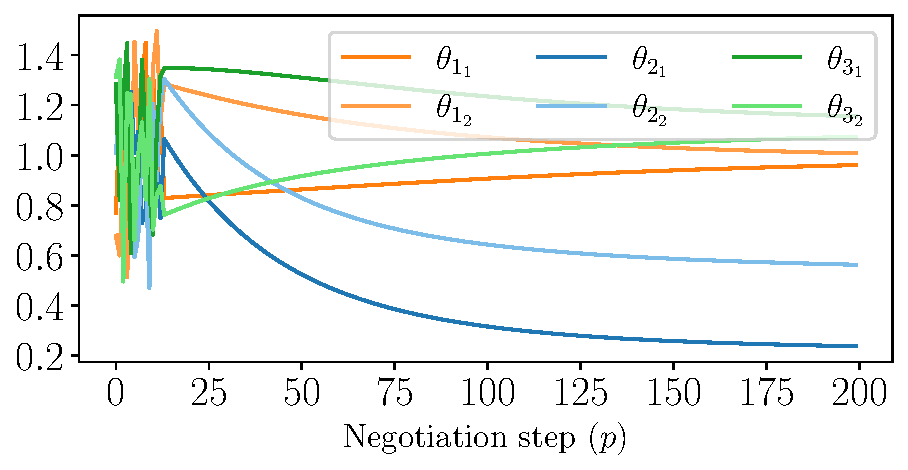
\includegraphics[width=.5\textwidth]{../img/resilient_eq/estimation_random_theta.pdf}
    \end{figure}
  \end{minipage}
  }
\end{frame}

\begin{frame}{Classification of mitigation techniques}
  \begin{itemize}
    \item Active (Resilient)
          \begin{enumerate}
            \item Detection/Isolation \onslide<1->{{\color{mpc_green}\faCheck}}
            \item Mitigation \onslide<2->{\color{mpc_agent}\faQuestionCircle}
          \end{enumerate}
  \end{itemize}
\end{frame}

\begin{frame}{Mitigation mechanism}{Reconstructing $\vec{\lambda}_{i}$}
  \begin{itemize}[<+->]
    \item Now, we have $\Plintildeestimate$
          \begin{itemize}
            \item Since $\Plintilde=\Tik\Plinnominal$
            \item We can recover $\Tik^{-1}$
          \begin{equation*}
            \widehat{\Tik^{-1}}=\Plin\Plintildeestimate^{-1}
          \end{equation*}
          \end{itemize}
    \item Reconstruct $\vec{\lambda}_{i}$
          \begin{equation*}
            \lambdaireconstructed=-\Plinnominal\thetai-\Tikinvestimate\siktildeestimate
          \end{equation*}
    \item Choose adequate version for coordination
          \begin{equation*}
            \lambdaimodified=
            \begin{cases}
              \lambdaireconstructed, &\text{if attack detected}\\
              \lambdaicheat, &\text{otherwise}\\
            \end{cases}
          \end{equation*}
  \end{itemize}
  \script<1->{Now, for the mitigation the main idea is to reconstruct the original lambda from the estimated parameters and use it in the negotiation\\ }
  \script<2->{We suppose the agent wants to decrease its cost, and the lambda sent is only equal to zero if the original is equal to zero. which implies the matrix T is invertible\\ }
  \script<3->{We can estimate the inverse of T, by using the estimate of P tilde and the nominal value of P like in this equation\\ }
  \script<4->{With the estimate of the inverse of T and the estimate of s tilde, we can reconstruct the original lambda\\ }
\end{frame}

\begin{frame}{Complete Mechanism}
  \begin{minipage}[c]{.35\linewidth}
    \begin{figure}[b]
      \centering
      \scalebox{.7}{
        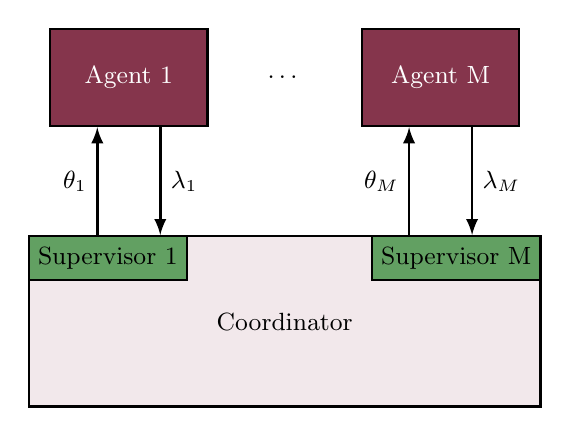
\begin{tikzpicture}[font=\small,thick,node distance=3*0.6180cm and 0.6180cm,every node/.style=rectangle,
          mpcSmall/.style={fill=mpc_agent, minimum height=0.6180*2cm, minimum width=2cm,text=white},
          coordinator/.style={fill=mpc_coordinator, minimum height=0.6180*3.5cm, minimum width=6.5cm},
          supervisor/.style={fill=mpc_green, minimum height=0.6180*3*0.3cm, minimum width=2cm},
          ]

          \node[draw, mpcSmall,] (block1) {\small Agent 1};
          \node[fill=none, draw=none, right=of block1,] (mult) {\bf $\dots$};
          \node[draw, mpcSmall, fill=mpc_agent, right=of mult,] (blockM) {\small Agent M};
          \node[draw, coordinator, below=of mult,] (coordinator) {Coordinator};

          \only<2->{\node[draw, supervisor,anchor=north west] at (coordinator.north west) {\small Supervisor 1};
          \node[draw, supervisor,anchor=north east] at (coordinator.north east) {\small Supervisor M};
}
          \draw[-latex,line width=1pt] (block1.south)+(0.4,.0) -- ( coordinator.north -| {$(block1.south)+(0.4,.0)$}) node [right,midway] {$\lambda_{1}$};
          \draw[latex-,line width=1pt] (block1.south)+(-0.4,0) -- (  coordinator.north -| {$(block1.south)+(-0.4,0)$}) node [left,midway] {$\theta_{1}$};
          \draw[-latex,line width=1pt] (blockM.south)+(0.4,.0) -- ( coordinator.north -| {$(blockM.south)+(0.4,.0)$}) node [right,midway] {$\lambda_{M}$};
          \draw[latex-,line width=1pt] (blockM.south)+(-0.4,0) -- (  coordinator.north -| {$(blockM.south)+(-0.4,0)$}) node [left,midway] {$\theta_{M}$};
        \end{tikzpicture}
      }
      % \caption{Scheme for Secure DMPC}\label{fig:schemeSafeQuantity}
    \end{figure}
  \end{minipage}
  % \pause
  \hfill
  \quad
  \hfill
  \begin{minipage}[c]{.6\linewidth}
    \begin{itemize}[<+(1)->]
      \item Supervise exchanges by inquiring the agents
      \item Estimate how they will behave
    \end{itemize}
    \pause Two Phases \pause
    \begin{enumerate}[<+->]
      \item Detect which agents are non-cooperative
      \item Reconstruct $\vec{\lambda}_{i}$ and use in negotiation
    \end{enumerate}
  \end{minipage}
  \script<1->{The complete mechanism is equivalent to add a supervisor for each agent inside the coordinator\\ }
  \script<2->{The mechanism is divided into the two phases, }
  \script<3->{first we detect which agents are non-cooperative }
  \script<4->{and then reconstruct the lambda i s and use in the usual negotiation\\ }
\end{frame}

\begin{frame}{Complete algorithm}{RPdMPC-DS}
  \begin{figure}[h]
    \centering
    \scalebox{.55}{
      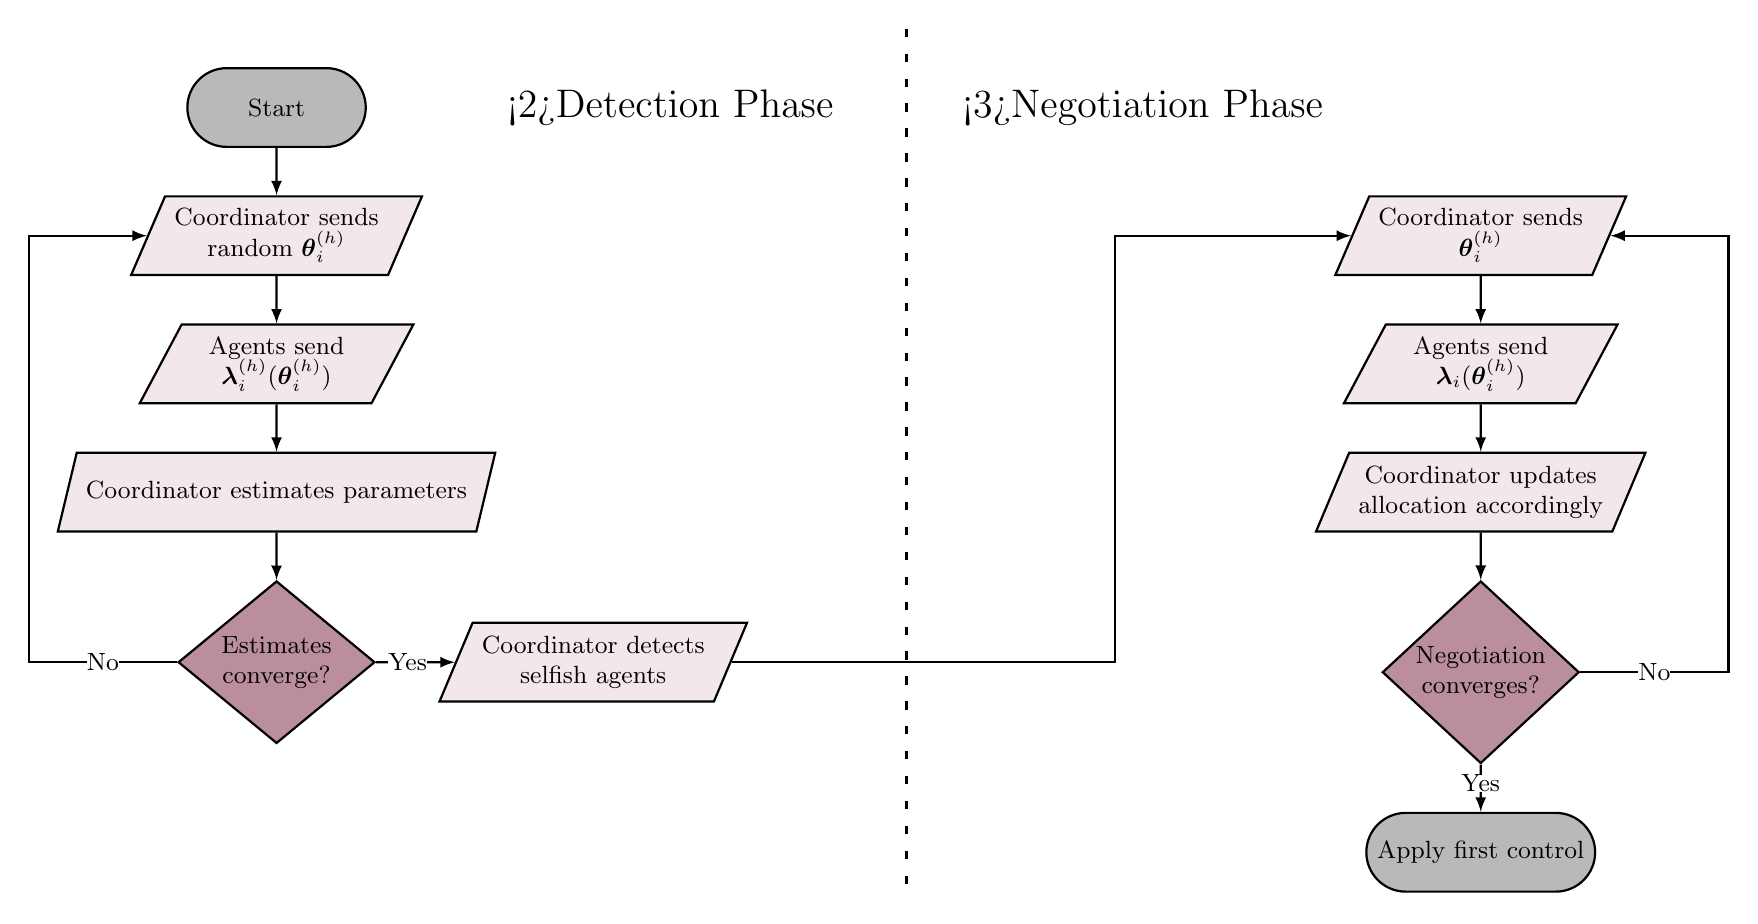
\begin{tikzpicture}[font=\small,thick,node distance=.6cm and 6cm]
        \draw[loosely dashed,
        minimum width=2.5cm,
        minimum height=1cm] (8cm,1cm) -- (8cm,-10cm);

        \node[] at (5cm,0cm) {\Large \alert<2>{Detection Phase}};
        \node[] at (11cm,0cm) {\Large \alert<3>{Negotiation Phase}};

        \node[draw,
        rounded rectangle,
        fill=gray!90!black!50,
        alt=<{4}>{fill=supelecRed!90,text=white},
        minimum width=2.5cm,
        minimum height=1cm] (block1) {Start};

        \node[draw,
        trapezium,
        trapezium left angle = 65,
        trapezium right angle = 115,
        trapezium stretches,
        align=center,
        fill=supelecRed!10,
        alt=<{5}>{fill=supelecRed!90,text=white},
        below=of block1,
        minimum width=3.5cm,
        minimum height=1cm
        ] (block2) { Coordinator sends \\random $\vec{\theta}_{i}^{(h)}$};

        \node[draw,
        trapezium,
        trapezium left angle = 65,
        trapezium right angle = 115,
        trapezium stretches,
        align=center,
        fill=supelecRed!10,
        alt=<{6}>{fill=supelecRed!90,text=white},
        below=of block2,
        minimum width=3.5cm,
        minimum height=1cm
        ] (block3) { Agents send \\ $\vec{\lambda}_{i}^{(h)}(\vec{\theta}_{i}^{(h)})$};

        \node[draw,
        trapezium,
        trapezium left angle = 65,
        trapezium right angle = 115,
        trapezium stretches,
        align=center,
        below=of block3,
        fill=supelecRed!10,
        alt=<{7}>{fill=supelecRed!90,text=white},
        minimum width=3.5cm,
        minimum height=1cm
        ] (block4) { Coordinator estimates parameters};

        \node[draw,
        diamond,
        below=of block4,
        minimum width=2.5cm,
        fill=supelecRed!50,
        alt=<{8}>{fill=supelecRed!90,text=white},
        align=center,
        inner sep=0] (block5) { Estimates\\ converge?};

        \node[draw,
        trapezium,
        trapezium left angle = 65,
        trapezium right angle = 115,
        trapezium stretches,
        align=center,
        fill=supelecRed!10,
        alt=<{9}>{fill=supelecRed!90,text=white},
        right=1cm of block5,
        minimum width=3.5cm,
        minimum height=1cm
        ] (block6) { Coordinator detects \\selfish agents};

        \node[coordinate,right=6.cm of block2] (block12) {};

        \node[draw,
        trapezium,
        trapezium left angle = 65,
        trapezium right angle = 115,
        trapezium stretches,
        align=center,
        right=of block12,
        fill=supelecRed!10,
        alt=<{10}>{fill=supelecRed!90,text=white},
        minimum width=3.5cm,
        minimum height=1cm
        ] (block7) { Coordinator sends \\$\vec{\theta}_i^{(h)}$};
        \node[draw,
        trapezium,
        trapezium left angle = 65,
        trapezium right angle = 115,
        trapezium stretches,
        align=center,
        fill=supelecRed!10,
        alt=<{11}>{fill=supelecRed!90,text=white},
        below=of block7,
        minimum width=3.5cm,
        minimum height=1cm
        ] (block8) { Agents send \\$\vec{\lambda}_i(\vec{\theta}_{i}^{(h)})$};

        \node[draw,
        trapezium,
        trapezium left angle = 65,
        trapezium right angle = 115,
        trapezium stretches,
        align=center,
        fill=supelecRed!10,
        alt=<{12}>{fill=supelecRed!90,text=white},
        below=of block8,
        minimum width=3.5cm,
        minimum height=1cm
        ] (block9) { Coordinator updates \\allocation accordingly};

        \node[draw,
        diamond,
        below=of block9,
        minimum width=2.5cm,
        fill=supelecRed!50,
        alt=<{13}>{fill=supelecRed!90,text=white},
        align=center,
        inner sep=0] (block10) { Negotiation\\ converges?};

        \node[draw,
        rounded rectangle,
        below=of block10,
        fill=gray!90!black!50,
        alt=<{14}>{fill=supelecRed!90,text=white},
        minimum width=2.5cm,
        minimum height=1cm,] (block11) { Apply first control};

        \draw[-latex] (block1) edge (block2)
        (block2) edge (block3)
        (block3) edge (block4)
        (block4) edge (block5);

        \draw[-latex] (block7) edge (block8)
        (block8) edge (block9)
        (block9) edge (block10);

        \draw[-latex] (block5) -- (block6)
        node[pos=0.4,fill=white,inner sep=0]{Yes};

        \draw[-latex] (block10) -- (block11)
        node[pos=0.4,fill=white,inner sep=0]{Yes};

        \draw[-latex] (block6) -| ($(block7.west) - (3cm,0)$) -- (block7.west);

        \draw[-latex] (block10) -| ($(block7.east) + (1.5cm,0)$)
        node[pos=0.25,fill=white,inner sep=0]{No} -- (block7.east);

        \draw[-latex] (block5) -| ($(block2.west) - (1.5cm,0)$)
        node[pos=0.25,fill=white,inner sep=0]{No} -- (block2.west);
      \end{tikzpicture}
    }
    % \caption{Secure DMPC}\label{fig:secureDMPC}
  \end{figure}
  \script<1->{Talk about RLS and convergence guaranteed, since it is linear and there is no noise. Now, for the complete secure DMPC algorithm, as said it is divided into two phases\\ }
  \script<2->{The Detection phase \\ }
  \script<3->{and the negotiation phase\\ }
  \script<5->{The coordinator sends random theta i\\ }
  \script<6->{The agents send dual variable lambda i\\ }
  \script<7->{The coordinator estimates the parameters P and s tilde\\ }
  \script<8->{when the estimates converge\\ }
  \script<9->{The coordinator detects which agents are non-cooperative\\ }
  \script<10->{then the negotiation phase begins, the coordinator sends the theta i\\ }
  \script<11->{the agents send the dual variable lambda i\\ }
  \script<12->{and the coordinator updates the allocation accordingly using the reconstructed lambda or the one sent by the agent\\ }
  \script<13->{and once the negotiation converges\\ }
  \script<14->{each agent applies the first control\\ }

\end{frame}

\subsection{Applying mechanism}

\begin{frame}{Example}
  \begin{minipage}[c]{.35\textwidth}
    \scalebox{0.5}{
      \begin{tikzpicture}[node distance=.5cm and .75cm,scale=1]
        \node[color=mpc_agent] (house1) at (0,0) {\scalebox{2.5}{\faHome}};
        \node[minimum height=1cm,below=of house1] (medium) {};
        \node[color=mpc_agent,right=of medium] (house2)  {\scalebox{3.5}{\faHome}};
        \node[color=mpc_agent,below=of medium] (house3)  {\scalebox{3}{\faHome}};
        \node[color=mpc_agent,left=3cm of medium] (house4)  {\scalebox{7}{\faHome}};

        \draw[latex-,line width=1pt] (house1) -- (medium.center);
        \draw[latex-,line width=1pt] (house2) -- (medium.center);
        \draw[latex-,line width=1pt] (house3) -- (medium.center);
        \draw[latex-,line width=1pt] (house4) -- (medium.center) node[above,midway] {\Huge $\vec{u}_{i}(t)$};
        \draw[color=black,fill=mpc_coordinator,] (medium) circle [radius=.2cm];

        \node[latex-,line width=7pt] at ($(house4) +(-1.5,1)$) {\Huge $w_{i}(t)$};
        \node[latex-,line width=7pt] at ($(house4) +(0,-1.5)$) {\Huge $\vec{x}_{i}(t)$};
        % \node[below=of house3] {$\left({\sum_{i=1}^{4} \vec{u}_{i}(k)\leq4\mathrm{kW}}\right)$};

      \end{tikzpicture}
    }
  \end{minipage}
  \hfill
  \begin{minipage}[c]{.6\textwidth}
    \begin{exampleblock}{District Heating Network (4 Houses)}
      \begin{itemize}[<+(1)->]
        \item Houses modeled using 3R-2C (monozone)
        \item Not enough power
        \item Period of ${5} \mathrm{h}$ ($T_{s}=0.25h$ $\to k=\{1\mathbin{:}20\}$)
        \item 3 scenarios
              \begin{itemize}
                \item[\encircle{N}] Nominal
                \item[\encircle{C}] Agent I cheats (dMPC)
                \item[\encircle{S}] Agent I cheats (RPdMPC-DS)
              \end{itemize}
        % \item $T_{1}=\left[\begin{smallmatrix}
  4 & 0 & 0 & 0\\
  0 & 4 & 0 & 0\\
  0 & 0 & 4 & 0\\
  0 & 0 & 0 & 4\\
\end{smallmatrix}
\right],\text{ if }k> 5$
      \end{itemize}
    \end{exampleblock}
  \end{minipage}
  \script<1->{We give an academic example of the temperature control of 4 distinct rooms under power scarcity\\}
  \script<2->{The 4 rooms are distinct using the 3 resistor 2 capacitor model\\}
  \script<3->{the initial temperature of all rooms is under 20 degrees celsius, which is the final setpoint\\}
  \script<4->{But they are under power scarcity that prevents them from reaching the setpoint\\}
  \script<5->{we simulate for a period of 5h\\}
  \script<6->{with sampling time of 15 minutes\\}
  \script<7->{3 scenarios are simulated, the nominal, one where agent 1 presents non cooperative behavior from k greater than 6, and another with the selfish behavior and the secure mechanism activated\\}
\end{frame}

\begin{frame}{Results}{Temporal}
  \centering
  \begin{minipage}[t]{.45\linewidth}
    \begin{figure}[h]
      \centering
      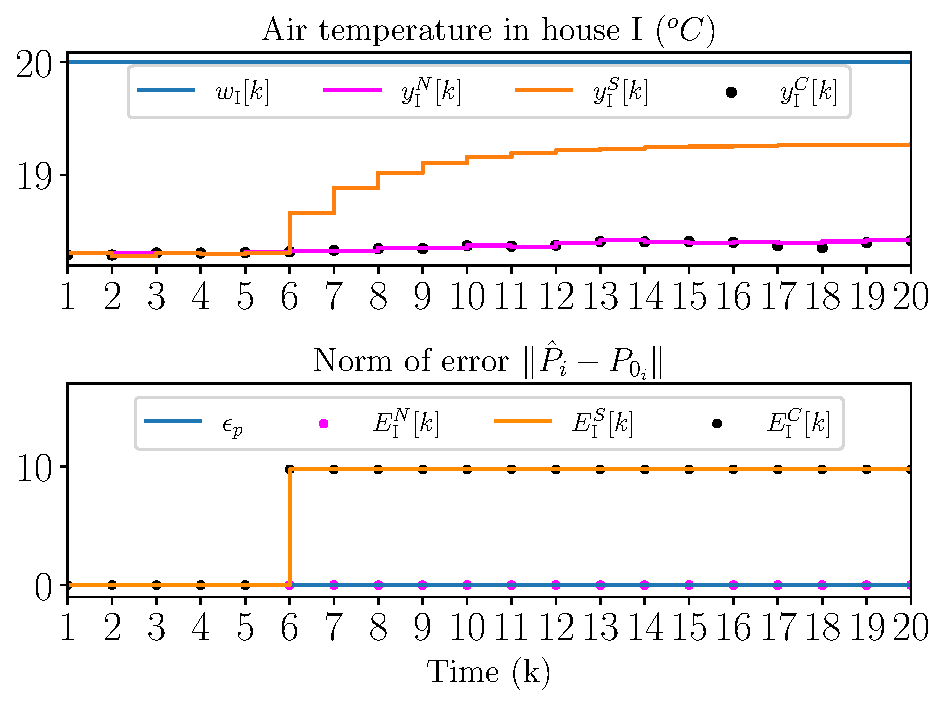
\includegraphics[width=1.\textwidth]{../img/resilient_eq/ErrorWX_command_normErrH.pdf}
      \caption*{Temperature in house I. \\Error $E_{I}(k)$.\\ {\encircle{N}} Nominal, {\encircle{S}} Selflish, {\encircle{C}} Corrected}
    \end{figure}
  \end{minipage}
  \only<2->{
  \begin{minipage}[t]{.50\linewidth}
    \begin{itemize}[<+(2)->]
      \item Agent starts cheating in $k=6$
      \item[\encircle{S}]  Agent increases its comfort
      \item[\encircle{C}] Restablish behavior close to \encircle{N}
    \end{itemize}
  \end{minipage}
  }
  \script<1>{In the figure we see the air temperature and the estimation error for house 1\\}
  \script<2>{When the room presents selfish behavior (in orange), it reduces its cost and get closer to the setpoint, we see that the attack increases the error\\}
  \script<3>{Now, for the case with correction (the black dots), even if it attacks the system, the temperature is close to its nominal value\\}
\end{frame}

\begin{frame}{Results}{Costs}
  \begin{table}[h]
    \centering
    \caption*{Objective functions $J_{i}$ (Normalized error \%)}\label{tab:eq_costsGlobalLocal}
    \begin{tabular}[t]{crr}
      \toprule
      Agent  & Selfish & Corrected\\
      \midrule
      I      &  $ -36.3 $ & $ 0.5  $\\
II     &  $ 21.67 $ & $ -0.55  $\\
III    &  $ 17.39 $ & $ -0.0  $\\
IV     &  $ 17.63 $ & $ -0.09  $\\
Global &  $ 3.53 $ & $ 0.02  $
\\
      \bottomrule
    \end{tabular}
  \end{table}
  \pause
  \script<1->{Now, if we compare the costs for each scenario we see how the cost of agent 1 decreases when it attacks, while the cost of other agents increase.\\}
  \script<2->{When the secure algorithm is activated the costs are very close to the original ones. So }
\end{frame}

\section{Resilient Primal Decomposition-based dMPC using Artificial Scarcity}
\subsection{Relaxing some assumptions}

\begin{frame}{Relaxing scarcity assumption}
  \begin{itemize}[<+(1)->]
    \item Systems are not completely deprived
          \begin{itemize}[<+(1)->]
            \item We can't change our constraints to equality ones anymore
            \item Nor use the simpler update equation
          \end{itemize}
  \end{itemize}

  \centering
  \onslide<.->{
    \begin{equation*}
      \begin{matrix}
        \minimize\limits_{\vec{U}_{i}[k]}&\frac{1}{2}\norm{\vec{U}_{i}[k]}^{2}_{H_{i}} + {\vec{f}_{i}[k]}^{T}\vec{U}_{i}[k]\\
        \mathrm{subject~ to} & \bar{\Gamma}_{i}\vec{U}_{i}[k] \preceq \thetaik:\lambdaik\\
      \end{matrix}
    \end{equation*}
  }
  \onslide<.(1)->{
    \begin{equation*}
      \vec{\theta}[k]\pplusone=\Proj^{\set{S}}(\vec{\theta}[k]\p+\rho\p\vec{\lambda}[k]\p)
    \end{equation*}
  }

  % \onslide<.(2)->{& \alert<.(2)>{\vec{U}_{i}[k]\in \set{U}_{i}}}
\end{frame}

\begin{frame}{Analyzing System}{Solution for $\lambda_{i}[k]$}
  \centering
  Instead of having one single affine solution
  \begin{equation*}
    \lambdaik=-\Plin\thetaik-\sik
  \end{equation*}
  \pause
  Now, we may have multiple \onslide<.(2)->{(Piecewise affine function)}
  \onslide<+(1)->{
    \begin{equation*}
      \small
      \hspace{-2cm}
      \begin{aligned}
        \lambdaik=
        \begin{cases}
          {-\Plinineq\thetaik-\sikineq},&\text{if}\ \thetaik \in\alert<.(2)>{\set{R}_{\lambdai}^{0}}\tikzmark{a}\\
          \qquad\quad \vdots&\qquad\quad \vdots\\
          -\Plinineq[i][2^{\nineq}-1]\thetaik-\sikineq[i][2^{\nineq}-1],&\text{if}\ \thetaik \in\alert<+(1)>{\set{R}_{\lambdai}^{2^{\nineq}-1}}\\
        \end{cases}
      \end{aligned}
    \end{equation*}
  }
  \onslide<+(1)->{
    \alert<+>{Still the $\Plinineq[i][n]$ are time independent}
  }
\end{frame}

\begin{frame}{Analyzing System}{Solution for $\lambda_{i}[k]$ (Continued)}
  \begin{figure}[h]
    \begin{tikzpicture}[every node/.style={align=center}]
      \def\height{3}
      \def\length{5}
      \node at (0,0) {} coordinate (p0)  ++(0:\length*2.2/5) coordinate (p1) ;
      \node at (0,0) {} ++(90:\height*2.8/5) coordinate (p2) ;

      \draw[black] (p2) ++(-4:5) coordinate (p3);
      \draw[black] (p1) ++(75:3) coordinate (p4);
      \coordinate (p6) at (p3|-p4);
      \coordinate (p5) at (intersection cs:first line={(p2)--(p3)}, second line={(p1)--(p4)});

      % \onslide\path[fill=gray!20] (p6) -- (p4) -- (p5) -- (p3);

      \only<8->{\onslide\path[fill=gray!20] (p1) -- (0,0) -- (p2) -- (p5);}

      \only<2->{
        \draw[black] (p2) -- (p3);
        \draw[black] (p1) -- (p4);
      }

      \draw[-latex] (0,-.1) - - (0,\height) node[left]{$\elem[2]{\thetai}$};
      \draw[-latex] (-.1,0) - - (\length,0) node[below]{$\elem[1]{\thetai}$};

      \onslide<4->{\draw[latex-] (-1,-.1) - - +(0,\height+.1) node[midway,rotate=90,anchor=center,yshift=.25cm]{Scarcity};
      \draw[latex-] (-.1,-.6) - - +(\length+.1,0) node[midway,below]{Scarcity};
      }

      \only<7->{\node at (\length*1.2/5,\height*1.25/5) {$\elem[1]{\lambdai}\neq0$\\$\elem[2]{\lambdai}\neq0$};}
      \only<6->{\node at (\length*1.2/5,\height*3.8/5) {$\elem[1]{\lambdai}=0$\\$\elem[2]{\lambdai}\neq0$};}
      \only<6->{\node at (\length*4/5,\height*1.25/5) {$\elem[1]{\lambdai}\neq0$\\$\elem[2]{\lambdai}=0$};}
      \only<5->{\node at (\length*4/5,\height*3.8/5) {$\elem[1]{\lambdai}=0$\\$\elem[2]{\lambdai}=0$};}

    \end{tikzpicture}
    % \caption*{Two constraints partitioning $\thetai$ solution space.}
  \end{figure}
  \centering
  \onslide<+(1)->{Separation surfaces depend on state and local parameters.}

  \onslide<+(1)->{Unknown by the coordinator.}

\end{frame}

\begin{frame}{Analyzing System}{Solution for $\lambda_{i}[k]$ (Continued) Still?}
  \centering
  \begin{equation*}
    \small
    \hspace{-2cm}
    \begin{aligned}
      \lambdaik=
      \begin{cases}
        \alert<4>{-\Plinineq\thetaik-\sikineq},&\text{if}\ \thetaik \in\set{R}_{\lambdai}^{0}\tikzmark{a}\\
        \qquad\quad \vdots&\qquad\quad \vdots\\
        \alert<5>{-\Plinineq[i][2^{\nineq}-1]\thetaik-\sikineq[i][2^{\nineq}-1]},&\text{if}\ \thetaik \in\set{R}_{\lambdai}^{2^{\nineq}-1}\\
      \end{cases}
    \end{aligned}
  \end{equation*}
  \onslide<2->{
    \begin{tikzpicture}[overlay, remember picture,decoration={brace,amplitude=2pt}]
      \draw[<-,thick] ($(a.north east) +(1,0)$) --+ (0,-2) node[midway, right=0.1cm,text=black,text width = 2in] {Scarcity};
    \end{tikzpicture}%
  }
  \onslide<3->{
    \begin{tikzpicture}[overlay, remember picture,decoration={brace,amplitude=2pt}]
      \draw[->,thick] ($(a.north east) +(3,0)$) --+ (0,-2) node[midway, right=0.1cm,text=black,text width = 2in] {Sparsity};
    \end{tikzpicture}%
  }
  \begin{equation*}
    \begin{matrix}
      \onslide<4->{
      \text{All constraints active}&-\Plinineq\thetaik-\sikineq & \to &-\Plin\thetaik-\sik \\
      }
      \onslide<5->{
      \text{None constraints active}&-\Plinineq[i][2^{\nineq}-1]\thetaik-\sikineq[i][2^{\nineq}-1] & \to & \0
                                                                          }
    \end{matrix}
  \end{equation*}

  \begin{minipage}[t]{.7\linewidth}

    \onslide<6->{
      \begin{assumptions}
        The region $\set{R}_{\lambdai}^{0}\neq \emptyset$ and we known a point $\thetairestricted\in\set{R}_{\lambdai}^{0}$
      \end{assumptions}
    }
  \end{minipage}
\end{frame}

\begin{frame}{Analyzing System}{Under attack!}
  \centering
  \vspace{-1cm}
  \onslide<+(1)->{
    \begin{equation*}
      \lambdaicheat[k]=\Tik\lambdai[k]
    \end{equation*}
  }
  \onslide<+(1)->{Parameters are modified.} \onslide<.(2)->{But not the regions' limits}

  \onslide<.(1)->{
  \begin{equation*}
    \small
      \lambdaicheat[k]=
      \begin{cases}
        -\Plinineqtilde      \thetaik-\sikineqtilde      ,&\text{if }\thetaik\in\set{R}^{0}\tikzmark{a}\\
        \qquad\quad \vdots&\qquad\quad \vdots\\
        -\Plinineqtilde[i][2^{\nineq}-1]\thetaik-\sikineqtilde[i][2^{\nineq}-1],&\text{if}\ \thetaik \in\set{R}_{\lambdai}^{2^{\nineq}-1}\\
      \end{cases}
  \end{equation*}
  }

  \begin{itemize}[<+(2)->]
    \item If we can estimate $\Plinineqtilde$ we can use same strategy than before
    \item Problem: We don't know in which region $\thetai$ is
    \item Solution: Let's force it using Artificial Scarcity
  \end{itemize}
\end{frame}

\subsection{Adapting the algorithm}

\begin{frame}{Artificial Scarcity}{Who is it? Who is it?}
  \centering
    \begin{itemize}
      \item<+(1)-> We use the point $\thetairestricted$, which activates all constraints\onslide<+(1)->{\footnote<.(1)->{If we have local constraints, we suppose this point respects them.}}
    \end{itemize}

  \onslide<+(1)->{
    \begin{minipage}[c]{.4\linewidth}
      \begin{figure}[h]
        \centering
        \scalebox{.9}{
          \begin{tikzpicture}[every node/.style={align=center}]
            \def\height{3}
            \def\length{5}
            \node at (0,0) {} coordinate (p0)  ++(0:\length*2.4/5) coordinate (p1) ;
            \node at (0,0) {} ++(90:\height*2.7/5) coordinate (p2) ;

            \draw[black] (p2) ++(-1:5) coordinate (p3);
            \draw[black] (p1) ++(80:3) coordinate (p4);
            \coordinate (p6) at (p3|-p4);

            \coordinate (p5) at (intersection cs:first line={(p2)--(p3)}, second line={(p1)--(p4)});
            \only<+->{\onslide\path[fill=gray!20] (p1) -- (0,0) -- (p2) -- (p5);}

            \draw[black] (p2) -- (p3);
            \draw[black] (p1) -- (p4);

            \draw[-latex] (0,-.1) - - (0,\height) node[left]{$\elem[2]{\thetai}$};
            \draw[-latex] (-.1,0) - - (\length,0) node[below]{$\elem[1]{\thetai}$};
            \only<-.>{
              \node at (\length*1.2/5,\height*1.25/5) {$\elem[1]{\lambdai}\neq0$\\$\elem[2]{\lambdai}\neq0$};
              \node at (\length*1.2/5,\height*3.8/5) {$\elem[1]{\lambdai}=0$\\$\elem[2]{\lambdai}\neq0$};
              \node at (\length*4/5,\height*1.25/5) {$\elem[1]{\lambdai}\neq0$\\$\elem[2]{\lambdai}=0$};
              \node at (\length*4/5,\height*3.8/5) {$\elem[1]{\lambdai}=0$\\$\elem[2]{\lambdai}=0$};
            }
            \only<.(3)-.(4)>{\node[draw,circle,minimum width=1cm] at (\length*.375,\height*0.3) {$\thetairestricted$};}
            \only<.(5)->{\node[draw,circle,minimum width=2.5cm] at (\length*.375,\height*0.3) {$\thetairestricted$};}
          \end{tikzpicture}
        }
      \end{figure}
    \end{minipage}
    \hfill
    \only<+(1)->{
      \begin{minipage}[c]{.55\linewidth}
        \begin{itemize}
          \item<+-> Generate points close to $\thetairestricted$
          \item<+(1)-> Estimate $\Plinineqtildeestimate$
        \end{itemize}
        \begin{itemize}
          \item<+(1)-> How do we known the radius?
                \begin{itemize}
                  \item<+(1)-> Unfortunately we don't.
                \end{itemize}
          \item<+(1)-> How to estimate $\Plinineqtildeestimate$ nonetheless?
        \end{itemize}
      \end{minipage}
    }
  }
\end{frame}

\begin{frame}{Enter Expectation Maximization}
  \begin{itemize}[<+(1)->]
    \item Iterative method to estimate parameters of multimodal models\onslide<+(1)->{\footnote<.(1)->{Such as our PWA function after using some tricks}}
  \end{itemize}

  \begin{itemize}[<+(1)->]
    \item We give multiple observations $\thetai^{o}[k]$ and $\lambdaicheat^{o}[k]$
    \item At each step we calculate
          \begin{enumerate}
            \item[\encircle{E}] the probability of each $(\Plinineqtildeestimate[i][n],\sikineqtildeestimate[i][n])$ having generated each $\lambdaicheat^{o}[k]$
            \item[\encircle{M}] new estimates $(\Plinineqtildeestimate[i][n],\sikineqtildeestimate[i][n])$ based on the probabilities
          \end{enumerate}
  \end{itemize}

  \begin{itemize}[<+(1)->]
    \item At the end we have
          \begin{enumerate}
            \item Parameters with associated region index
            \item Observations with associated region index
          \end{enumerate}
    \item We consult the index associated to $\thetairestricted$
    \item We recover the associated parameter, i.e., $\Plinineqtildeestimate$
  \end{itemize}
\end{frame}

\begin{frame}{Detection and Mitigation}{Same same, but different}

  \onslide<+(1)->{
    \begin{assumption}
      We estimate nominal $\Plinineqnominal$ from attack free negotiation
    \end{assumption}
  }

  \begin{itemize}[<+(1)->]
    \item Detection
          \begin{equation*}
            \norm{\Plinineqtildeestimate-\Plinineqnominal}_{F} \geq\epsilon_{\Plinineq}
          \end{equation*}
    \item Mitigation
          \onslide<+->{
          \begin{equation*}
            {\Tikinvestimate=\Plinineqnominal{\Plinineqtildeestimate}^{-1}}.
          \end{equation*}
          }
          \onslide<+->{
          \begin{equation*}
            \lambdaireconstructed=\Tikinvestimate \lambdaicheat.
          \end{equation*}
          }
  \end{itemize}
\end{frame}

\begin{frame}{Complete algorithm}{RPdMPC-AS}
  \begin{figure}[h]
    \centering
  \scalebox{.55}{
    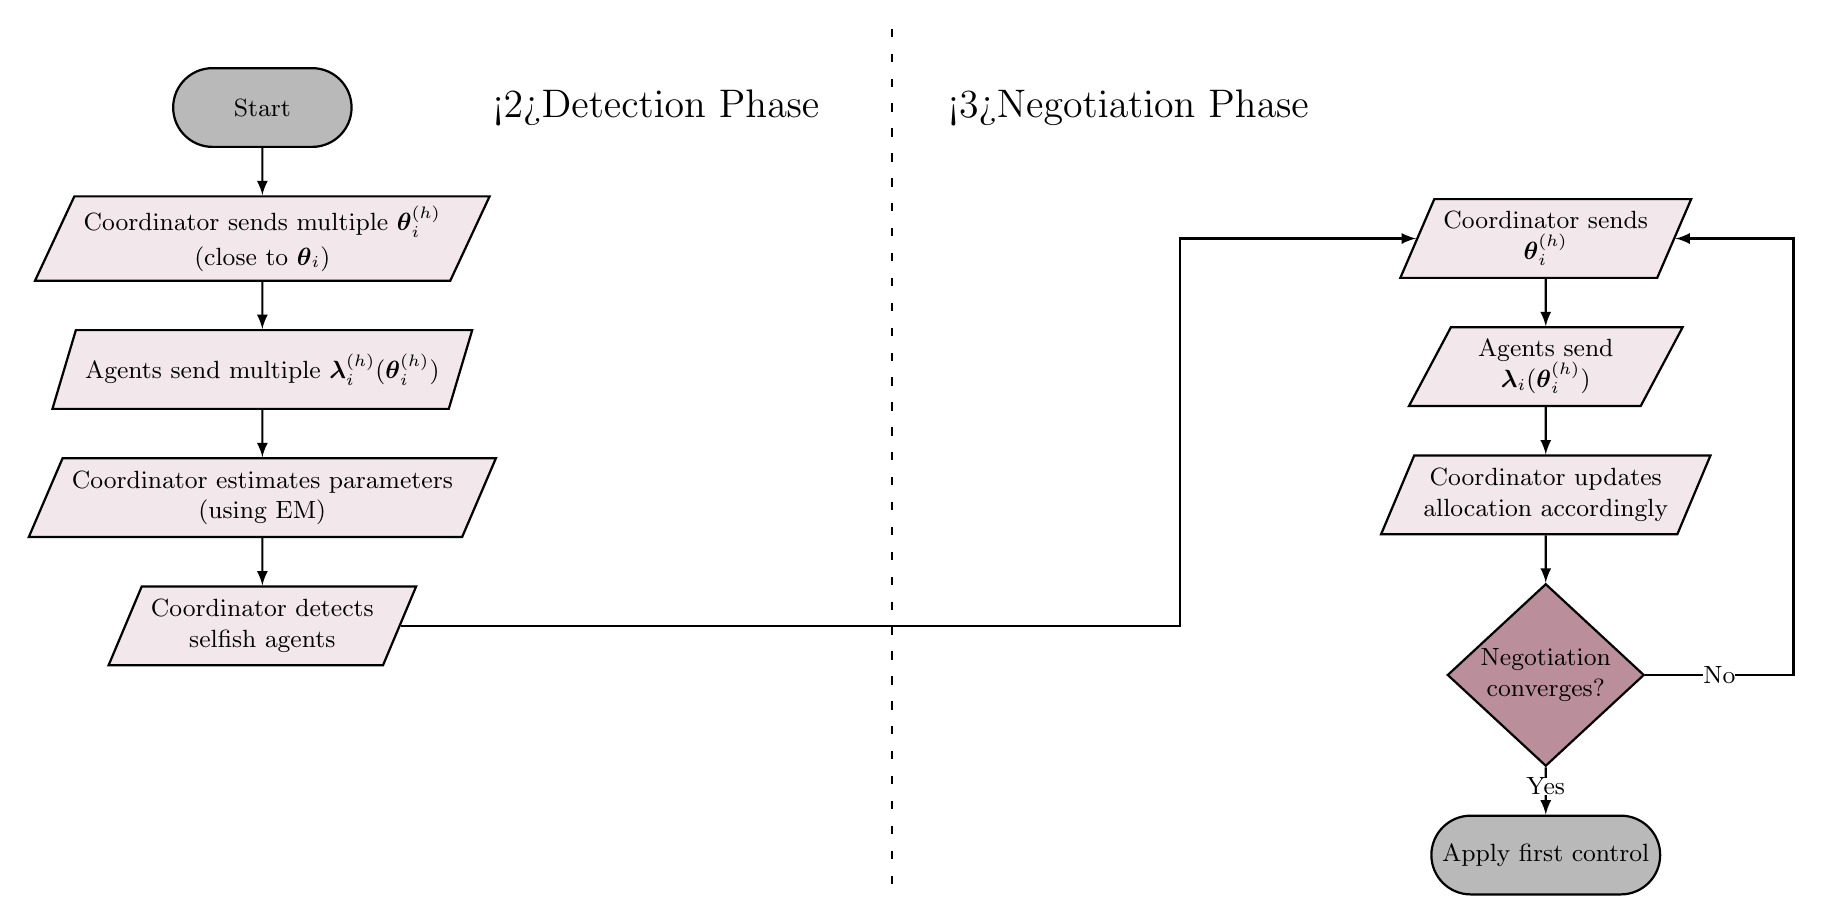
\begin{tikzpicture}[font=\small,thick,node distance=.6cm and 6cm]
      \draw[loosely dashed,
      minimum width=2.5cm,
      minimum height=1cm] (8cm,1cm) -- (8cm,-10cm);

      \node[] at (5cm,0cm) {\Large \alert<2>{Detection Phase}};
      \node[] at (11cm,0cm) {\Large \alert<3>{Negotiation Phase}};

      \node[draw,
      rounded rectangle,
      fill=gray!90!black!50,
      % alt=<{4}>{fill=supelecRed!90,text=white},
      minimum width=2.5cm,
      minimum height=1cm] (block1) {Start};

      \node[draw,
      trapezium,
      trapezium left angle = 65,
      trapezium right angle = 115,
      trapezium stretches,
      align=center,
      fill=supelecRed!10,
      alt=<{4}>{fill=supelecRed!90,text=white},
      below=of block1,
      minimum width=3.5cm,
      minimum height=1cm
      ] (block2) { Coordinator sends multiple $\vec{\theta}_{i}^{(h)}$\\ (close to $\thetairestricted$)};

      \node[draw,
      trapezium,
      trapezium left angle = 65,
      trapezium right angle = 115,
      trapezium stretches,
      align=center,
      fill=supelecRed!10,
      alt=<{4}>{fill=supelecRed!90,text=white},
      below=of block2,
      minimum width=3.5cm,
      minimum height=1cm
      ] (block3) { Agents send multiple $\vec{\lambda}_{i}^{(h)}(\vec{\theta}_{i}^{(h)})$};

      \node[draw,
      trapezium,
      trapezium left angle = 65,
      trapezium right angle = 115,
      trapezium stretches,
      align=center,
      below=of block3,
      fill=supelecRed!10,
      alt=<{4}>{fill=supelecRed!90,text=white},
      minimum width=3.5cm,
      minimum height=1cm
      ] (block4) { Coordinator estimates parameters\\
      (using EM)};

      % \node[draw,
      % diamond,
      % below=of block4,
      % minimum width=2.5cm,
      % fill=supelecRed!50,
      % alt=<{8}>{fill=supelecRed!90,text=white},
      % align=center,
      % inner sep=0] (block5) { Estimates\\ converge?};

      \node[draw,
      trapezium,
      trapezium left angle = 65,
      trapezium right angle = 115,
      trapezium stretches,
      align=center,
      fill=supelecRed!10,
      % alt=<{8}>{fill=supelecRed!90,text=white},
      below=of block4,
      minimum width=3.5cm,
      minimum height=1cm
      ] (block5) { Coordinator detects \\selfish agents};

      \node[coordinate,right=6.cm of block2] (block12) {};

      \node[draw,
      trapezium,
      trapezium left angle = 65,
      trapezium right angle = 115,
      trapezium stretches,
      align=center,
      right=of block12,
      fill=supelecRed!10,
      % alt=<{9}>{fill=supelecRed!90,text=white},
      minimum width=3.5cm,
      minimum height=1cm
      ] (block7) { Coordinator sends \\$\vec{\theta}_i^{(h)}$};
      \node[draw,
      trapezium,
      trapezium left angle = 65,
      trapezium right angle = 115,
      trapezium stretches,
      align=center,
      fill=supelecRed!10,
      % alt=<{10}>{fill=supelecRed!90,text=white},
      below=of block7,
      minimum width=3.5cm,
      minimum height=1cm
      ] (block8) { Agents send \\$\vec{\lambda}_i(\vec{\theta}_{i}^{(h)})$};

      \node[draw,
      trapezium,
      trapezium left angle = 65,
      trapezium right angle = 115,
      trapezium stretches,
      align=center,
      fill=supelecRed!10,
      alt=<{5}>{fill=supelecRed!90,text=white},
      below=of block8,
      minimum width=3.5cm,
      minimum height=1cm
      ] (block9) { Coordinator updates \\allocation accordingly};

      \node[draw,
      diamond,
      below=of block9,
      minimum width=2.5cm,
      fill=supelecRed!50,
      % alt=<{12}>{fill=supelecRed!90,text=white},
      align=center,
      inner sep=0] (block10) { Negotiation\\ converges?};

      \node[draw,
      rounded rectangle,
      below=of block10,
      fill=gray!90!black!50,
      % alt=<{13}>{fill=supelecRed!90,text=white},
      minimum width=2.5cm,
      minimum height=1cm,] (block11) { Apply first control};

      \draw[-latex] (block1) edge (block2)
      (block2) edge (block3)
      (block3) edge (block4)
      (block4) edge (block5);

      \draw[-latex] (block7) edge (block8)
      (block8) edge (block9)
      (block9) edge (block10);

      % \draw[-latex] (block5) -- (block6)
      % node[pos=0.4,fill=white,inner sep=0]{Yes};

      \draw[-latex] (block10) -- (block11)
      node[pos=0.4,fill=white,inner sep=0]{Yes};

      \draw[-latex] (block5) -| ($(block7.west) - (3cm,0)$) -- (block7.west);

      \draw[-latex] (block10) -| ($(block7.east) + (1.5cm,0)$)
      node[pos=0.25,fill=white,inner sep=0]{No} -- (block7.east);

      % \draw[-latex] (block5) -| ($(block2.west) - (1.5cm,0)$)
      % node[pos=0.25,fill=white,inner sep=0]{No} -- (block2.west);
    \end{tikzpicture}
    }
    % \caption{Secure DMPC}\label{fig:secureDMPC}
  \end{figure}

\end{frame}

\subsection{Applying mechanism}

\begin{frame}{Example}
  \begin{minipage}[c]{.35\textwidth}
    \scalebox{0.5}{
      \begin{tikzpicture}[node distance=.5cm and .75cm,scale=1]
        \node[color=mpc_agent] (house1) at (0,0) {\scalebox{2.5}{\faHome}};
        \node[minimum height=1cm,below=of house1] (medium) {};
        \node[color=mpc_agent,right=of medium] (house2)  {\scalebox{3.5}{\faHome}};
        \node[color=mpc_agent,below=of medium] (house3)  {\scalebox{3}{\faHome}};
        \node[color=mpc_agent,left=3cm of medium] (house4)  {\scalebox{7}{\faHome}};

        \draw[latex-,line width=1pt] (house1) -- (medium.center);
        \draw[latex-,line width=1pt] (house2) -- (medium.center);
        \draw[latex-,line width=1pt] (house3) -- (medium.center);
        \draw[latex-,line width=1pt] (house4) -- (medium.center) node[above,midway] {\Huge $\vec{u}_{i}(t)$};
        \draw[color=black,fill=mpc_coordinator,] (medium) circle [radius=.2cm];

        \node[latex-,line width=7pt] at ($(house4) +(-1.5,1)$) {\Huge $w_{i}(t)$};
        \node[latex-,line width=7pt] at ($(house4) +(0,-1.5)$) {\Huge $\vec{x}_{i}(t)$};
        % \node[below=of house3] {$\left({\sum_{i=1}^{4} \vec{u}_{i}(k)\leq4\mathrm{kW}}\right)$};

      \end{tikzpicture}
    }
  \end{minipage}
  \hfill
  \begin{minipage}[c]{.6\textwidth}
    \begin{exampleblock}{District Heating Network (4 Houses)}
      \begin{itemize}
        \item Houses modeled using 3R-2C
        \item \only<1>{Not enough power}\only<2->{\st{Not enough power} (Change $(\vec{x}_{0},\vec{w}_{0})$)}
        \item Period of ${5} \mathrm{h}$ ($T_{s}=0.25h$ $\to k=\{1\mathbin{:}20\}$)
        \item 3 scenarios
              \begin{itemize}
                \item[\encircle{N}] Nominal
                \item[\encircle{C}] Agent I cheats (dMPC)
                \item[\encircle{S}] Agent I cheats (RPdMPC-AS)
              \end{itemize}
      \end{itemize}
    \end{exampleblock}
  \end{minipage}
\end{frame}

\begin{frame}{Results}{Temporal}
  \centering
  % \begin{minipage}[c]{.45\linewidth}
  \begin{overlayarea}{1\textwidth}{.5\textwidth}
  \begin{figure}[h]
    \centering
    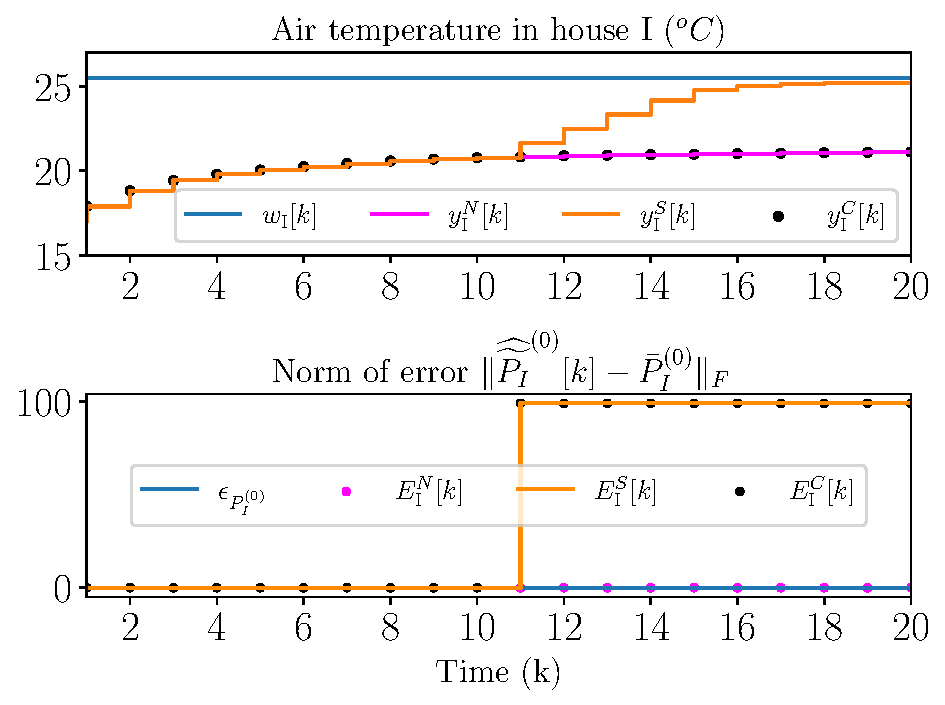
\includegraphics[width=.45\textwidth,trim=0 .3cm 0 .2cm,clip]{../img/resilient_ineq/ErrorWX_command_normErrH.pdf}
    \caption*{Temperature in house I. \\Error  $E_{I}(k)$.\\ {\encircle{N}} Nominal, {\encircle{S}} Selflish {\encircle{C}} Corrected}
  \end{figure}

  \only<2->{
    \begin{tikzpicture}[overlay, remember picture]
      \node at (12.,4.5) {
        \reflectbox{
\includegraphics[width=.25\textwidth,trim=0 .3cm 0 .2cm,clip]{../img/mutley.jpg}}
      };
    \end{tikzpicture}%
  }

  \end{overlayarea}

\end{frame}

% \begin{frame}{Results}{Temporal (Continued)}
%   \begin{figure}[h]
%     \centering
%     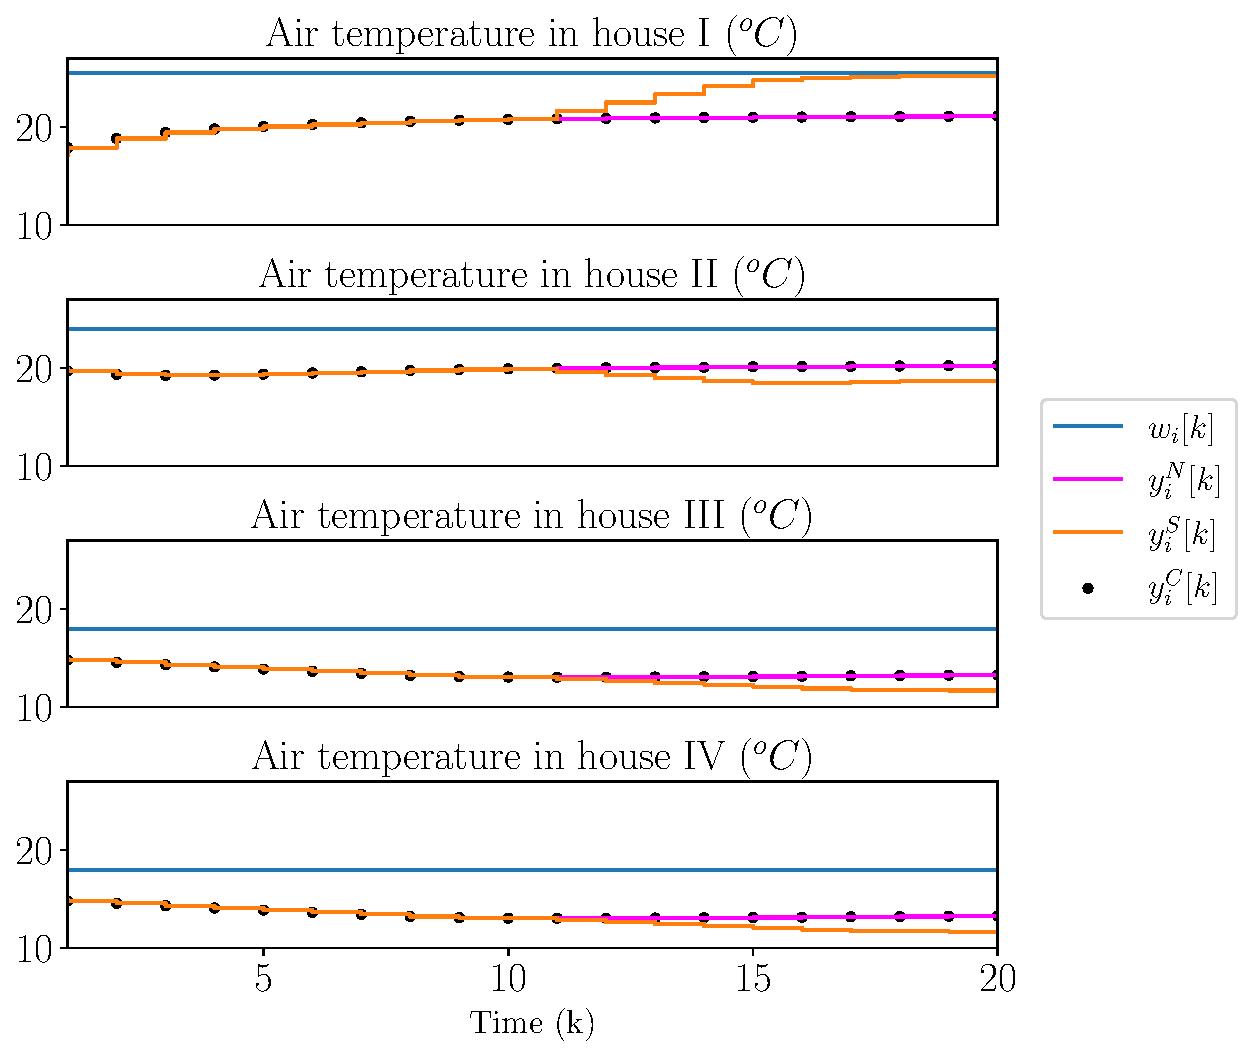
\includegraphics[width=.5\textwidth,trim=0 .3cm 0 .2cm,clip]{../img/resilient_ineq/ErrorWX_command_normErrH_all_houses.pdf}
%     \caption*{Air temperature in all houses for different scenarios. \\ {\encircle{N}} Nominal, {\encircle{S}} Selflish behavior, {\encircle{C}} Selfish + Correction}
%   \end{figure}
% \end{frame}

% \begin{frame}{Results}{Control}
%   \begin{figure}[h]
%     \centering
%      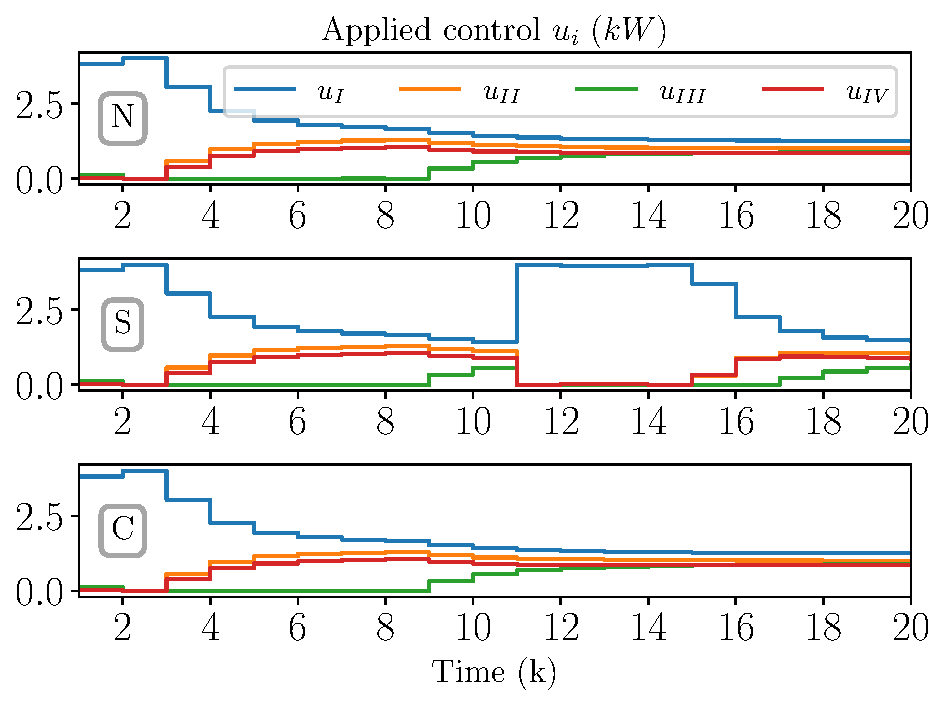
\includegraphics[width=.5\textwidth,trim=0 .1cm 0 .3cm,clip]{../img/resilient_ineq/control.pdf}
%     \caption*{Control applied in all houses for different scenarios. \\ {\encircle{N}} Nominal, {\encircle{S}} Selflish behavior, {\encircle{C}} Selfish + Correction}
%   \end{figure}
% \end{frame}

\begin{frame}{Results}{Costs}
  \begin{table}[h]
    \centering
    \caption*{Objective functions $J_{i}$ (Normalized error \%)}\label{tab:eq_costsGlobalLocal}
    \begin{tabular}[t]{crr}
      \toprule
      Agent  & Selfish & Corrected\\
      \midrule
      I      &  $ -36.489 $ & $ -0.0  $\\
II     &  $ 35.813 $ & $ 0.0  $\\
III    &  $ 29.225 $ & $ 0.0  $\\
IV     &  $ 37.541 $ & $ 0.0  $\\
Global &  $ 10.689 $ & $ -0.0  $
\\
      \bottomrule
    \end{tabular}
  \end{table}
\end{frame}

\begin{frame}{Too good to be true!}{\only<1>{It's a kind of magic!}\only<2->{\st{It's a kind of magic!}}}
  \begin{itemize}[<+(1)->]
    \item Unfortunately EM is not magic
          \begin{itemize}
            \item Slow convergence
            \item Dependency on initialization
                  \begin{itemize}
                    \item No guarantees of achieving global optimal
                  \end{itemize}
          \end{itemize}
    \item Some ``solutions'':
          \begin{itemize}
            \item Force some parameters to converge faster (case dependant)
            \item Run multiple times with different initialization and pick best
            \item Associate with other methods of the same family
          \end{itemize}
  \end{itemize}
\end{frame}

\section{Conclusion}

\begin{frame}{Conclusion}{Main takeaways}
  \begin{itemize}
    \item How can an agent attack? \onslide<2->{{\color{mpc_green} \faCheck}}
  \begin{itemize}
    \item<2-> Attacker can change the communication to receive more ressources.
  \end{itemize}
    \item What are the consequences of an attack? \onslide<3->{{\color{mpc_green} \faCheck}}
  \begin{itemize}
    \item<3-> Suboptimality and maybe instability
  \end{itemize}
    \item Can we mitigate the effects? \onslide<4->{{\color{mpc_green} \faCheck}}
  \begin{itemize}
          \item<4-> Yes! By exploring the scarcity of the systems!
  \end{itemize}
  \end{itemize}
\end{frame}

\begin{frame}{Conclusion}{Recap}
  \begin{itemize}[<+(1)->]
    \item Insights from the analysis of the solutions of the optimization problems:
          \begin{itemize}
            \item Sensibilities are constant when there is no cheating
            \item They may change when system is attacked
          \end{itemize}

    \item Exploiting the scarcity of resources, we find how to invert the attack
          \begin{itemize}
            \item Straightforward if system is completely deprived
            \item If not, we try to force it artifically
                  \begin{itemize}
                    \item However, solution is PWA and we need special estimation method
                  \end{itemize}
          \end{itemize}
  \end{itemize}

  \begin{itemize}[<+(1)->]
    \item What if complete scarcity information is not available? \onslide<+(1)->{Not even artificially?}
  \end{itemize}

  \visible<+(1)->{
    \begin{figure}[h]
      \centering
      
\includegraphics[width=.4\textwidth]{back_to_future.png}
    \end{figure}
  }
\end{frame}

\begin{frame}{Open question Future Directions}
    \begin{itemize}[<+->]
      \item Reconstruction of cheating matrix with partial/incremental scarcity
      \item Study of robustness/Error Propagation + noise
      \item Resilient strategy with soft constraints 
      \item Recursive EM (or alternative)
      \item ...
    \end{itemize}
\end{frame}

\appendix

\begin{frame}[plain]
  \centering
  \vfill
  Questions? Comments?
  \vfill
  \begin{minipage}[t]{.45\linewidth}
    \small
    \centering
    Repository
    \href{https://github.com/Accacio/thesis}{https://github.com/Accacio/thesis}

    
\includegraphics[width=2cm]{qrRepo.png}
  \end{minipage}
  \hfill
  \begin{minipage}[t]{.5\linewidth}
    \small
    \centering
    Contact\\
    \href{mailto:rafael.accacio.nogueira@gmail.com?subject=Thesis Defense Presentation}{rafael.accacio.nogueira@gmail.com}

    
\includegraphics[width=2cm]{qrContact.png}
  \end{minipage}
  \ifwebcast{\tikz{\draw[fill=pink,draw=pink] (1.5,0) circle [radius=1.5cm]}}%
  \fi
      \script{If you want to see the simulations of this paper we have a github repository, and if you want to send me an email about this paper or this presentation you can flash the QR code in the right. Thank you!\\}

\end{frame}

\begin{frame}[allowframebreaks]
% \bibliographystyle{apalike}
% \bibliography{../tex/bibliography}
  \frametitle<presentation>{For Further Reading}

%   \begin{thebibliography}{10}

%   \beamertemplatebookbibitems % Start with overview books.
%   \bibitem{MaestreEtAl2014}
%   J.~M. Maestre, R.~R. Negenborn \emph{et~al.}
%   \newblock \emph{{D}istributed {M}odel {P}redictive {C}ontrol made easy}.\hskip 1em plus 0.5em minus 0.4em\relax
%   \newblock Springer, 2014, vol.~69.

%   \beamertemplatearticlebibitems
%   % Followed by interesting articles. Keep the list short.

% \bibitem{VelardeEtAl2017a}
% P.~Velarde, J.~M. Maestre, H.~Ishii, and R.~R. Negenborn,
% \newblock ``Scenario-based
% defense mechanism for distributed model predictive control,''
% \newblock \emph{2017
%   IEEE 56th Annual Conference on Decision and Control (CDC)}.\hskip 1em plus
%   0.5em minus 0.4em\relax IEEE, Dec 2017, pp. 6171--6176.
\setbeamertemplate{bibliography item}[book]
\printbibliography[type=book,title={Books}]
\setbeamertemplate{bibliography item}[article]
\printbibliography[type={article},title={Articles}]
\printbibliography[type={inproceedings},title={Articles}]
% \end{thebibliography}

    \script{As a recommended reading I give a book about distributed MPC and an article with another secure dmpc algorithm based in another decomposition method. That's all\\}
\end{frame}

\begin{frame}{Conditions}{\hyperlink{analysis_deprived_systems}{\beamerreturnbutton{back}}}
  \hypertarget{condition_transform_equality}{}

  One way to ensure this, is to make the original constraints to form a cone.

  \vspace{1cm}
  \begin{minipage}[c]{.3\linewidth}
    \begin{figure}[H]
      \centering
      \scalebox{0.9}{
        \begin{tikzpicture}
          \def\ang{-35}
          \def\vecmag{.25}
          \node at (0,0) {} coordinate(p1) ++(\ang:2.5) coordinate(p2) ++(\ang-90:1.5) coordinate(p3) ++(\ang-180:2.5) coordinate(p4);

          \path (p1) -- (p2) coordinate[pos=-0.2](a1l) coordinate[pos=1.2](a1r) coordinate[pos=0.8](m12);
          \draw[-latex] (a1l) -- (m12) -- ([turn] -90:0.5) node[left]{$\vec{\eta}_1$};
          \draw  (m12) -- (a1r);

          \path (p3) -- (p4) coordinate[pos=-0.2](a3l) coordinate[pos=1.2](a3r) coordinate[pos=0.8](m34);
          \draw[-latex] (a3l) -- (m34) -- ([turn] -90:0.5) node[right]{$\vec{\eta}_2$};
          \draw  (m34) -- (a3r);

        \end{tikzpicture}
      }
      \caption*{No intersection}\label{fig:non_feasible}
    \end{figure}
  \end{minipage}
  \hfill
  \begin{minipage}[c]{.3\linewidth}
    \begin{figure}[h]
      \centering
      \scalebox{0.9}{
        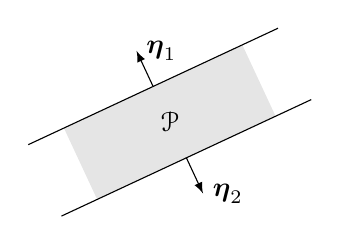
\begin{tikzpicture}
          \def\ang{25}
          \def\vecmag{.5}
          \node at (0,0) {} coordinate(p1) ++(\ang:2.5) coordinate(p2) ++(\ang-90:1.) coordinate(p3) ++(\ang-180:2.5) coordinate(p4);
          \path[fill=gray!20] (p1) -- (p2) -- (p3) -- (p4);
          \node at (barycentric cs:p1=1,p2=1,p3=1,p4=1) {$\mathcal{P}$};

          \path (p1) -- (p2) coordinate[pos=-0.2](a1l) coordinate[pos=1.2](a1r) coordinate[pos=0.5](m12);
          \draw[-latex] (a1l) -- (m12) -- ([turn] 90:0.5) node[right]{$\vec{\eta}_1$};
          \draw  (m12) -- (a1r);

          \path (p3) -- (p4) coordinate[pos=-0.2](a3l) coordinate[pos=1.2](a3r) coordinate[pos=0.5](m34);
          \draw[-latex] (a3l) -- (m34) -- ([turn] 90:0.5) node[right]{$\vec{\eta}_2$};
          \draw  (m34) -- (a3r);
        \end{tikzpicture}
      }
      \caption*{$\vecangle{\vec{\eta}_{1}}{\vec{\eta}_{2}}=180^{o}$}\label{fig:parallel_only_one_active}
    \end{figure}
  \end{minipage}
  \hfill
  \begin{minipage}[c]{.3\linewidth}
    \begin{figure}[h]
      \centering
      \scalebox{0.9}{
        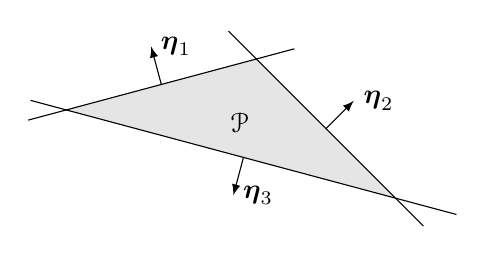
\begin{tikzpicture}
          \node at (0,0) {} coordinate(p1) ++(15:2.5) coordinate(p2) ++(-45:2.5) coordinate(p3) ++ (-195:4.0) coordinate(p4);
          \path[fill=gray!20] (p1) -- (p2) -- (p3);
          \node at (barycentric cs:p1=1,p2=1,p3=1) {$\mathcal{P}$};

          \foreach \X [count=\Y] in {2,...,4}
          {
            \path (p\Y) -- (p\X) coordinate[pos=-0.2](a\Y{}l) coordinate[pos=1.2](a\Y{}r) coordinate[pos=0.5](m\Y\X);
            \draw[-latex] (a\Y{}l) -- (m\Y\X) -- ([turn]90:.5) node[right]{$\vec{\eta}_\Y$};
            \draw (m\Y\X) -- (a\Y{}r);
          }
        \end{tikzpicture}
      }
      \caption*{A $3$-sided polyhedron.}\label{fig:triangle_inequality}
    \end{figure}
  \end{minipage}

\end{frame}

\begin{frame}{$\theta$ dynamics}{\hyperlink{analysis_continued}{\beamerreturnbutton{back}}}
  \hypertarget{theta_dynamics}{}
  \begin{equation*}
    \vec{\theta}\pplusone=\mathcal{A}_{\theta}\vec{\theta}\p+\mathcal{\vec{B}}_{\theta}[k]
  \end{equation*}
  where
  \begin{equation*}
    \mathcal{A}_{\theta}=\left[
      \begin{matrix}
        I-\frac{M-1}{M}\rho\p \Plin[1] & \frac{1}{M}\rho\p \Plin[2]&\dots&\frac{1}{M}\rho\p \Plin[M]\\
        \frac{1}{M}\rho\p \Plin[1]&I-\frac{M-1}{M}\rho\p \Plin[2]&\dots&\frac{1}{M}\rho\p \Plin[M]\\
        \vdots&\vdots&\ddots&\vdots\\
        \frac{1}{M}\rho\p \Plin[1]&\frac{1}{M}\rho\p \Plin[2]&\dots&I-\frac{M-1}{M}\rho\p \Plin[M]\\
      \end{matrix}
    \right]
  \end{equation*}
  \begin{equation*}
    \mathcal{\vec{B}}_{\theta}[k]=\left[
      \begin{matrix}
        -\frac{M-1}{M}\rho\p \vec{s}_{1}[k]+\frac{1}{M}\rho\p \vec{s}_{2}[k]\dots-\frac{1}{M}\rho\p \vec{s}_{M}[k]\\
        \frac{1}{M}\rho\p \vec{s}_{1}[k]-\frac{M-1}{M}\rho\p \vec{s}_{2}[k] \dots-\frac{1}{M}\rho\p \vec{s}_{M}[k]\\
        \vdots\\
        \frac{1}{M}\rho\p \vec{s}_{1}[k]+\frac{1}{M}\rho\p \vec{s}_{2}[k]\dots-\frac{M-1}{M}\rho\p \vec{s}_{M}[k]\\
      \end{matrix}
    \right]
  \end{equation*}
\end{frame}

\end{document}
